\chapter{Multiple Populations in NGC 2808}\label{chap:ngc2808}

Globular clusters (GCs) are among the oldest observable objects in the universe
\citep{Pen11}. They are characterized by high densities with typical half-light
radii of $\le$10 pc \citep{Vanderburg2010}, and typical masses ranging from
$10^{4}$--$10^{5}$ M$_{\odot}$ \citep{Bro06} --- though some GCs are
significantly larger than these typical values \citep[e.g. $\omega$Cen,
][]{Richer1991}. GCs provide a unique way to probe stellar evolution
\citep{Bau03}, galaxy formation models \citep{Boy18,Kra05}, and dark matter
halo structure \citep{Hud18}. Further, globular cluster ages provide 
independent constraints on cosmological models \citep[e.g.][]{Vandenberg1996, Cunha2002, Krauss2003, Trenti2015, Valcin2021, Ying2023}.

The traditional view of Globular Clusters was, for a long time, that they
consisted of a single stellar population (SSP, in some publications this is
referred to as a Simple Stellar Population). This view was supported by
spectroscopically uniform heavy element abundances \citep{Carretta2010,
Bastian2018} accross most clusters (M54 and $\omega$Cen are notable exceptions,
see \citet{Marino2015} for further details), and the lack of evidence for
multiple stellar populations (MPs) in past color-magnitude diagrams of GCs
\citep[i.e.][]{Sandage1953, Alcaino1975}. However, over the last 40 years
non-trivial star-to-star light-element abundance variations have been observed
\citep[i.e.][]{Smith1987} and, in the last two decades, it has been
definitively shown that most if not all Milky Way GCs have MPs
\citep{Gratton2004, Gratton2012, Piotto2015}. The lack of photometric evidence
for MPs can be attributed to the short color throw available to ground based
photometric surveys \citep{Milone2017}; specifically, lacking UV filters. While
MPs are chemically distinct from one another, that distinction is most
prominent when observing with $U$ and $B$ filters \citep{Sbordone2011}.

The prevalence of multiple populations in GCs is so distinct that the proposed
definitions for what constitutes a globular cluster now often center the
existence of MPs. Whereas, people have have often tried to categorized objects
as GCs through relations between half-light radius, density, and surface
brightness profile, in fact many objects which are generally thought of as GCs
don't cleanly fit into these cuts \citep{Peebles1968, Brown1991, Brown1995, Bekki2002}.
Consequently, \citet{Carretta2010} proposed a definition of GC based on
observed chemical inhomogeneities in their stellar populations. The modern
understanding of GCs then is not simply one of a dense cluster of stars which
may have chemical inhomogeneities and multiple populations; rather, it is one
where those chemical inhomogeneities and multiple populations themselves are
the defining element of a GC.

All Milky Way globular clusters studied in detail show populations enriched in
He, N, and Na while also being deplete in O and C
\citep{Piotto2015,Bastian2018}. Further, studies of Magellenic Cloud
massive clusters have shown that these light element abundance variations exist
in clusters as young as $\sim 2$ Gyr but not in younger clusters
\citep{Martocchia2019} while there is also evidence of nitrogen variability in
the $\sim 1.5$ Gyr old cluster NGC 1783 \citep{Cadelano2022}.  These light
element abundance patterns also are not strongly correlated with variations in
heavy element abundance, resulting in spectroscopically uniform Fe abundances
between populations \citep[though recent work indicates that there may be
iron abundance variations within the first population, e.g.][]{Legnardi2022,
Lardo2022} . Further, high-resolution spectral studies reveal anti-correlations
between N-C abundances, Na-O abundances, and potentially Al-Mg
\citep{Sneden1992, Gratton2012}. Typical stellar fusion reactions can deplete
core oxygen; however, the observed abundances of Na, Al, and Mg cannot be
explained by the CNO cycle \citep{Prantzos2007}. Consequently, globular cluster
populations must be formed by some novel means.

Formation channels for these multiple populations remain a point of debate
among astronomers. Most proposed formation channels consist of some older,
more massive, population of stars polluting the pristine cluster media before a
second population forms, now enriched in heavier elements which they themselves could
not have generated \citep[for a detailed review see ][]{Gratton2012}. The four
primary candidates for these polluters are asymptotic giant branch stars
\citep[AGBs,][]{Ventura2001,DErcole2010}, fast rotating massive stars
\citep[FRMSs,][]{Decressin2007}, super massive stars
\citep[SMSs,][]{Denissenkov2014}, and massive interacting binaries
\citep[MIBs,][]{deMink2009, Bastian2018}. 

Hot hydrogen burning (proton capture), material transport to the surface, and
material ejection into the intra-cluster media are features of each of these
models and consequently they can all be made to {\it qualitatively} agree with
the observed elemental abundances. However, none of the standard models can
currently account for all specific abundances \citep{Gratton2012}. AGB and FRMS
models are the most promising; however, both models have difficulty reproducing
severe O depletion \citep{Ventura2009,Decressin2007}. Moreover, AGB and FRMS
models require significant mass loss ($\sim 90\%$) between cluster formation
and the current epoch --- implying that a significant fraction of halo stars
formed in GCs \citep{Renzini2008,DErcole2008,Bastian2015}.

In addition to the light-element anti-correlations observed it is also known
that younger populations are significantly enhanced in Helium
\citep{Piotto2007, Piotto2015, Latour2019}. Depending on the cluster, Helium
mass fractions as high as $Y=0.4$ have been inferred \citep[e.g][]{Milone2015}.
However, due to the relatively high and tight temperature range of partial
ionization for He it cannot be observed in globular clusters; consequently, the
evidence for enhanced He in GCs originates from comparison of theoretical
stellar isochrones to the observed color-magnitude-diagrams of globular
clusters. Therefore, a careful handling of chemistry is essential when modeling
with the aim of discriminating between MPs; yet, only a very limited number of
GCs have yet been studied with chemically self-consistent (structure and
atmosphere) isochrones \citep[e.g.][NGC 6752]{Dotter2015}. 

% \chapter{Modeling Globular Clusters}
% Due to the importance of globular clusters accross domains of astronomy 
% there are multiple ways to model them. Some of these approaches, for work
% which is primarily focused on teh dynamics of clusters and galxies, treat
% globular clusters as dynamical systems and study aspects such as evaporation rates
% and dynamical cooling timescales. 

% An analytic framework for understanding cluster evaporation was proposed by
% both \citet{Amb38} and \citet{Spi40}, who suggested an expression for a
% dimensionless evaporation rate $\xi$.
% \begin{equation}
%     \xi \equiv -\frac{t_{rh}}{M}\frac{dM}{dt}
% \end{equation}
% where $M$ is the total cluster mass and the relaxation time $t_{rh}$ is defined as:
% \begin{equation}
%     t_{rh} = \frac{0.14 N}{\ln\Lambda}\sqrt{\frac{r^{3}_{hm}}{GM}}
% \end{equation}
% Where $r_{hm}$ is the half mass radius of the cluster. Additionally, $\Lambda
% \equiv 0.4N$ and N is the total number of stars in the cluster. Due to the
% complexity of cluster mass evaporation, the initial attempts to analytically
% constrain the value of $\xi$ have been superseded by numerical calculations. As
% a result, it has since been shown that both external tidal fields \citep{Mad17,
% Bau03} and stellar evolution \citep{Bau03} play important roles in determining
% a cluster's mass loss rate.

% Understanding the evaporation and expansion history of GCs can shed light on
% both the galactic potentials in which the cluster lives, and where the cluster
% formed in the galactic potential \citep{Ren17}. \citet{Wil03} and \citet{Gon05}
% presented early evidence via numeric studies that the primordial binary
% fraction of a cluster may influence a cluster's core radius expansion rate.
% Their results show that a direct proportionality between the binary fraction
% and core radius expansion rates may exist. Further, \citet{Lan07} provided
% empirical evidence, through a study of blue straggler stars (BSS) in M5, that
% collisional binaries may increase evaporation rates. However, there has yet to
% be established a firm quantitative relationship between the primordial binary
% fraction of a cluster and its evolutionary rates

\section{Introduction}\label{sec:Intro}
Globular clusters (GCs) are among the oldest observable objects in the universe
\citep{Pen11}. They are characterized by high densities with typical half-light
radii of $\le$10 pc \citep{Vanderburg2010}, and typical masses ranging from
$10^{4}$--$10^{5}$ M$_{\odot}$ \citep{Bro06} --- though some GCs are
significantly larger than these typical values \citep[e.g. $\omega$ Cen,
][]{Richer1991}. GCs provide a unique way to probe stellar evolution
\citep{Bau03}, galaxy formation models \citep{Boy18,Kra05}, and dark matter
halo structure \citep{Hud18}.

The traditional view of Globular Clusters was that they consisted of a single
stellar population (SSP, in some publications this is referred to as a Simple
Stellar Population). This view was supported by spectroscopically uniform heavy
element abundances \citep{Carretta2010, Bastian2018} across most clusters (M54
and $\omega$Cen are notable exceptions, see \citet{Marino2015} for further
details), and the lack of evidence for multiple stellar populations (MPs) in
past color-magnitude diagrams of GCs \citep[i.e.][]{Sandage1953, Alcaino1975}.
However, over the last 40 years non-trivial star-to-star light-element
abundance variations have been observed \citep[i.e.][]{Smith1987} and, in the
last two decades, it has been definitively shown that most if not all Milky Way
GCs have MPs \citep{Gratton2004, Gratton2012, Piotto2015}. The lack of
photometric evidence for MPs prior to the 2000, can be attributed to the more
narrow color bands available, until very recently, to ground based photometric
surveys \citep{Milone2017}.

The prevalence of multiple populations in GCs is so distinct that the proposed
definitions for what constitutes a globular cluster now often center the
existence of MPs \citep[e.g.][]{Carretta2010}. Whereas, people have have often
tried to categorized objects as GCs through relations between half-light
radius, density, and surface brightness profile, in fact many objects which are
generally thought of as GCs don't cleanly fit into these cuts
\citep{Peebles1968, Brown1991, Brown1995, Bekki2002}. Consequently,
\citet{Carretta2010} proposed a definition of GC based on observed chemical
inhomogeneities in their stellar populations. The modern understanding of GCs
then is not simply one of a dense cluster of stars that may have chemical
inhomogeneities and multiple populations; rather, it is one where those
chemical inhomogeneities and multiple populations themselves are the defining
element of a GC.

All Milky Way globular clusters studied in detail show populations enriched in
He, N, and Na while also being deplete in O and C
\citep{Piotto2015,Bastian2018}. {\bf Further, studies of Magellenic Cloud
massive clusters have shown that these light element abundance variations exist
in clusters as young as $\sim 2$ Gyr but not in younger clusters
\citep{Martocchia2019} while there is also evidence of nitrogen variability in
the $\sim 1.5$ Gyr old cluster NGC 1783 \citep{Cadelano2022}}.  These light
element abundance patterns also are not strongly correlated with variations in
heavy element abundance, resulting in spectroscopically uniform Fe abundances
between populations \citep[{\bf though recent work indicates that there may be
[Fe/H] variations within the first population, e.g.}][]{Legnardi2022,
Lardo2022} . Further, high-resolution spectral studies reveal anti-correlations
between N-C abundances, Na-O abundances, and potentially Al-Mg
\citep{Sneden1992, Gratton2012}. Typical stellar fusion reactions can deplete
core oxygen; however, the observed abundances of Na, Al, and Mg cannot be
explained by the CNO cycle \citep{Prantzos2007}. Consequently, globular cluster
populations must be formed by some novel means.

Formation channels for these multiple populations remain a point of debate
among astronomers. Most proposed formation channels consist of some older,
more massive, population of stars polluting the pristine cluster media before a
second population forms, now enriched in heavier elements which they themselves could
not have generated \citep[for a detailed review see ][]{Gratton2012}. The four
primary candidates for these polluters are asymptotic giant branch stars
\citep[AGBs,][]{Ventura2001,DErcole2010}, fast rotating massive stars
\citep[FRMSs,][]{Decressin2007}, super massive stars
\citep[SMSs,][]{Denissenkov2014}, and massive interacting binaries
\citep[MIBs,][]{deMink2009, Bastian2018}. 

Hot hydrogen burning (i.e. proton capture), material transport to the surface, and
material ejection into the intra-cluster media are features of each of these
models and consequently they can all be made to {\it qualitatively} agree with
the observed elemental abundances. However, none of the standard models can
currently account for all specific abundances \citep{Gratton2012}. AGB and FRMS
models are the most promising; however, both models have difficulty reproducing
severe O depletion \citep{Ventura2009,Decressin2007}. Moreover, AGB and FRMS
models require significant mass loss ($\sim 90\%$) between cluster formation
and the current epoch --- implying that a significant fraction of halo stars
formed in GCs \citep{Renzini2008,DErcole2008,Bastian2015}.

In addition to the light-element anti-correlations observed, it is also known
that second populations are significantly enhanced in Helium
\citep{Piotto2007, Piotto2015, Latour2019}. Depending on the cluster, helium
mass fractions as high as $Y=0.4$ have been inferred \citep[e.g][]{Milone2015}.
However, due to both the relatively high and tight temperature range of partial
ionization for He and the efficiency of gravitational settling in core helium
burning stars, the initial He abundance of globular cluster stars cannot be
observed; consequently, the evidence for enhanced He in GCs originates from
comparison of theoretical stellar isochrones to the observed
color-magnitude-diagrams of globular clusters. Therefore, a careful handling of
chemistry is essential when modeling with the aim of discriminating between
MPs; yet, only a very limited number of GCs have been studied with
chemically self-consistent (structure and atmosphere) isochrones
\citep[e.g.][NGC 6752]{Dotter2015}. 

NGC 2808 is the prototype globular cluster to host Multiple Populations.
Various studies since 2007 have identified that it may host anywhere from 2-5
stellar populations. These populations have been identified both
spectroscopically \citep[i.e.][]{Carretta2004, Carretta2006, Carretta2010,
Gratton2011, Carretta2015, Hong2021} and photometrically
\citep[i.e.][]{Piotto2007, Piotto2015, Milone2015, Milone2017, Pasquato2019}.
Note that recent work \citep{Valle2022} calls into question the statistical
significance of the detections of more than 2 populations in the spectroscopic
data. Here we present new, chemically self-consistent modeling of the
photometry of the two extreme populations of NGC 2808 identified by
\citet{Milone2015}, populations A and E. {\bf We do not consider populations B,
C, or D identified in \citet{Milone2015} as the purpose of this work is to
identify if chemically self-consistent modelling results in a statisically
signifigant deviation in the infered helium abundance when compared to non
chemically self-consistent models. Use of the two populations in the NGC 2808
with the highest identified difference between their helium populations is
sufficent for to answer this question.}  We use archival photometry from the
Hubble UV Globular Cluster Survey (HUGS) \citep{Piotto2015, Milone2017} in the
F275W and F814W passbands to characterize multiple populations in NGC 2808
\citep{Milone2015, Milone2015b} (This data is avalible at MAST: \href{https://archive.stsci.edu/doi/resolve/resolve.html?doi=10.17909/T9810F}{10.17909/T9810F}). Additionally, we present a
likelihood analysis of the photometric data of NGC 2808 to determine the number
of populations present in the cluster.



\input{chapters/ngc2808/subsections/observations}
\section{Modeling}\label{sec:modeling}
One of the most pressing questions related to this work is whether or not the
increased star-to-star variability in the activity metric and the Jao Gap,
which are coincident in magnitude, are driven by the same underlying mechanism.
The challenge when addressing this question arises from current computational
limitations. Specifically, the kinds of three dimensional
magneto-hydrodynamical simulations --- which would be needed to derive the
effects of convective kissing instabilities on the magnetic field of the star
--- are unfeasible to run over gigayear timescales while maintaining thermal
timescale resolutions needed to resolve periodic mixing events.

In order to address this and answer the specific question of \textit{could
kissing instabilities result in increased star-to-star variability of the
magnetic field}, we adopt a very simple toy model. Kissing instabilities result
in a transient radiative zone separating the core of a star (convective) from its
envelope (convective). When this radiative zone breaks down two important
things happen: one, the entire star becomes mechanically coupled, and two,
convective currents can now move over the entire radius of the star.
\citet{Jao2023} propose that this mechanical coupling may allow the star's core
to act as an angular momentum sink thus accelerating a stars spin down and
resulting in anomalously low H$\alpha$ emission. 

Regardless of the exact mechanism by which the magnetic field may be affected,
it is reasonable to expect that both the mechanical coupling and the change to
the scale of convective currents will have some effect on the star's magnetic
field. On a microscopic scale both of these will change how packets of charge
within a star move and may serve to disrupt a stable dynamo. Therefore, in the
model we present here we make only one primary assumption: \textit{every mixing
event may modify the star's magnetic field by some amount}. Within our model
this assumption manifests as a random linear perturbation applied to some base
magnetic field at every mixing event. The strength of this perturbation is 
sampled from a normal distribution with some standard deviation, $\sigma_{B}$.

Synthetic stars are sampled from a grid of stellar models evolved using the
Dartmouth Stellar Evolution Program (DSEP) with similar parameters to those
used in \citet{Boudreaux2023}. Each stellar model was evolved using a high
temporal resolution (timesteps no larger than 10,000 years) and typical
numerical tolerances of one part in $10^5$. Each model was based on a GS98
\citep{Grevesse1998} solar composition with a mass range from 0.3 M$_{\odot}$
to 0.4 M$_{\odot}$. Finally, models adopt OPLIB high temperature radiative
opacities, Ferguson 2004 low temperature radiative opacities, and include both
atomic diffusion and gravitational settling. A Kippenhan-Iben diagram showing
the structural evolution of a model within the Gap is shown in Figure
\ref{fig:kippenhan}.

\begin{figure*}
  \centering
  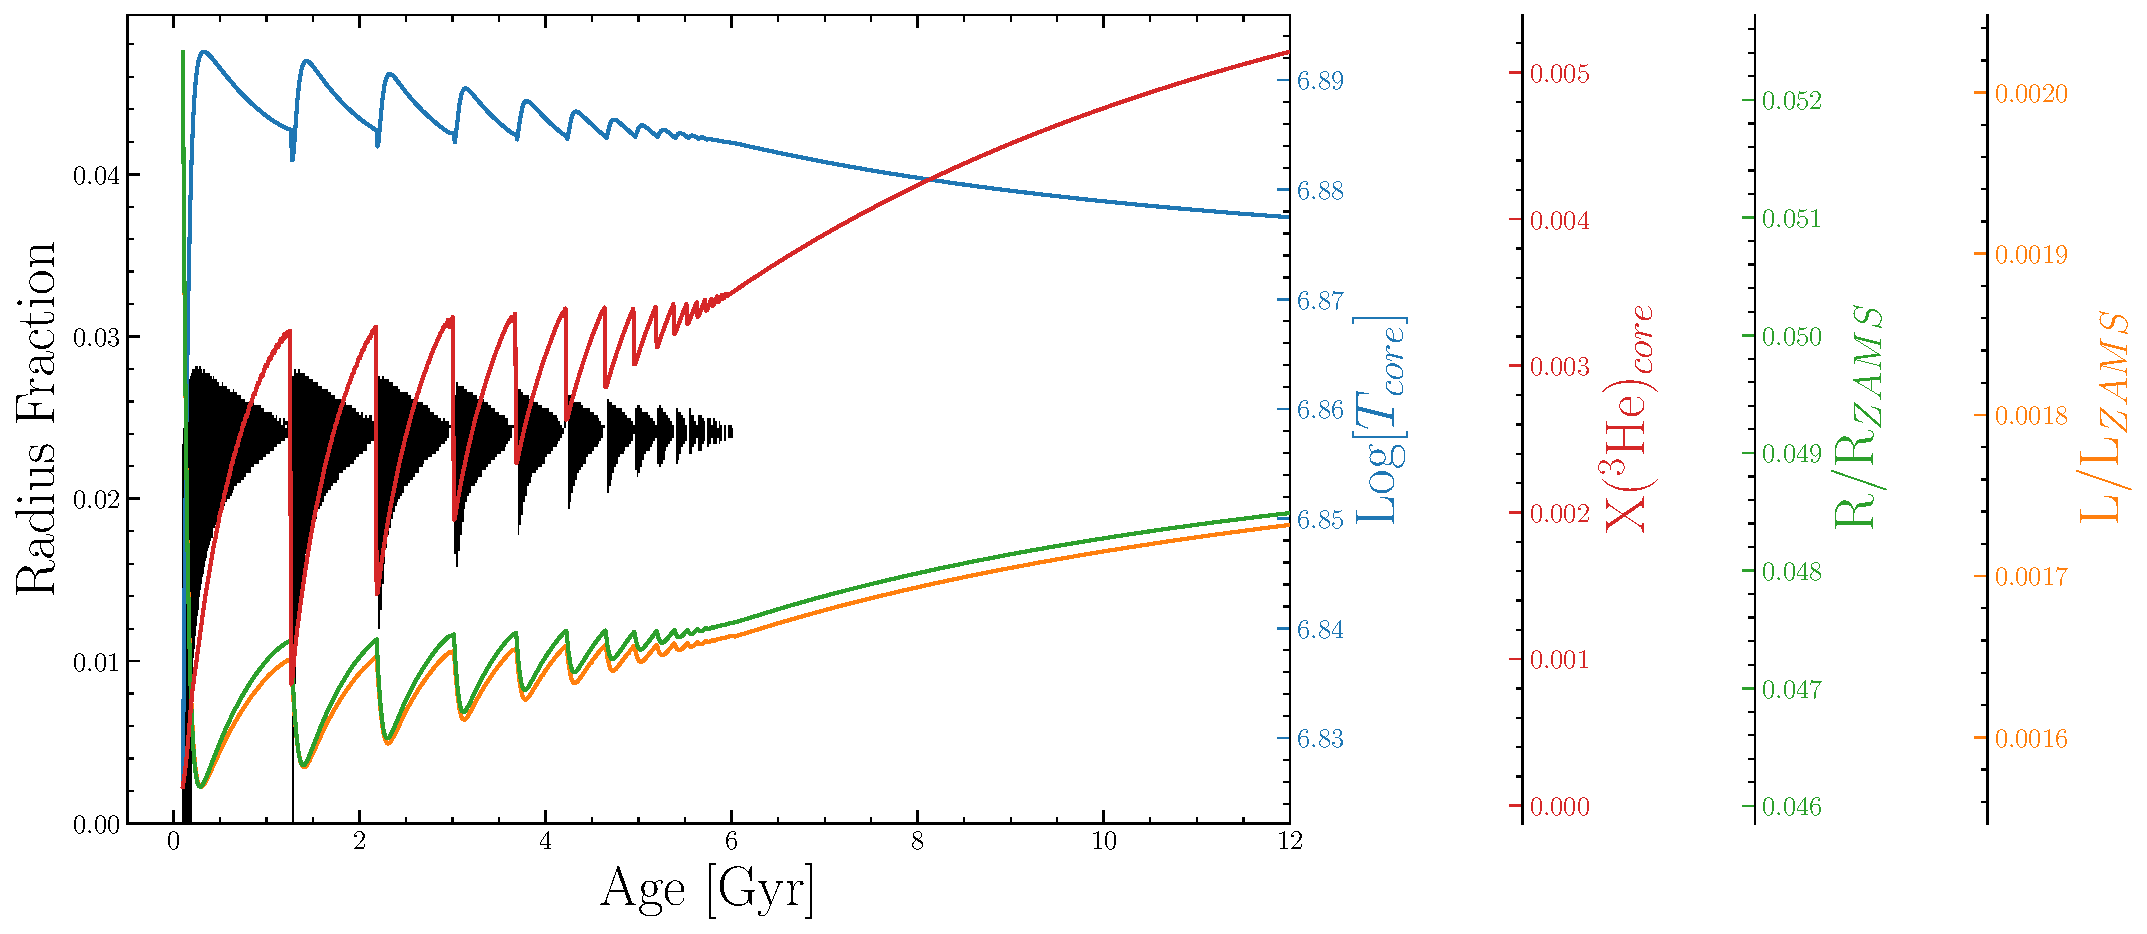
\includegraphics[width=0.9\textwidth]{figures/jaoMagActivity/Kippenhan_clamped.pdf}
  \caption{Kippenhan-Iben diagram for a 0.345 solar mass star. Note the
  periodic mixing events (where the plotted curves peak).}
  \label{fig:kippenhan}
\end{figure*}

Each synthetic star is assigned some base magnetic activity ($B_{0} \sim
\mathcal{N}(1, \sigma_{B})$) and then the number of mixing events before some age $t$
are counted based on local maxima in the core temperature. The toy magnetic
activity at age $t$ for the model is given in Equation \ref{eqn:activity}. An
example of the magnetic evolution resulting from this model is given in Figure
\ref{fig:simpleB}. Fundamentally, this model presents magnetic
activity variation due to mixing events as a random walk and therefore results will
increasing divergence over time.

\begin{align}\label{eqn:activity}
  B(t) = B_{0} + \sum_{i}B_{i} \sim \mathcal{N}(1, \sigma_{B}) 
\end{align}

\begin{figure}
  \centering
  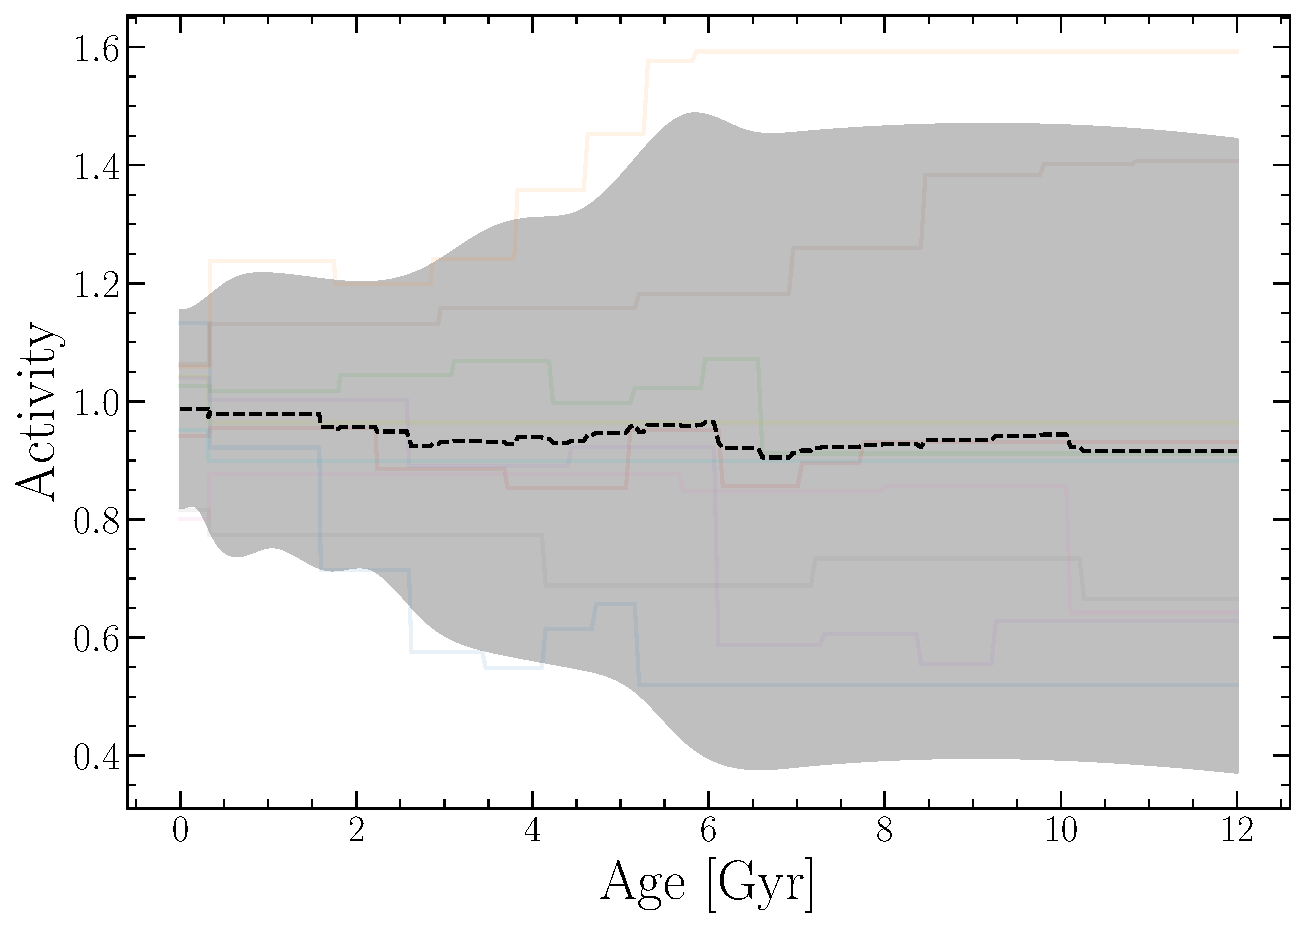
\includegraphics[width=0.85\textwidth]{figures/jaoMagActivity/simpleBEvolution.pdf}
  \caption{Example of the toy model presented here resulting in increased
  divergence between stars magnetic fields. The shaded region represents the
  maximum spread in the two point correlation function at each age.}
  \label{fig:simpleB}
\end{figure}

Applying the same analysis to these models as was done to the observations as
described in Section \ref{sec:results} we find that this simple model results
in a qualitatively similar trend in the standard deviation vs. Magnitude graph
(Figure \ref{fig:model}). In order to reproduce the approximately 50 percent
change to the spread of the activity metric observed in the combined dataset in
section \ref{sec:results} a distribution with a standard deviation of 0.1 is
required when sampling the change in the magnetic activity metric at each
mixing event. This corresponds to 68 percent of mixing events modifying the
activity strength by 10 percent or less. The interpretation here is important:
what this qualitative similarity demonstrates is that it may be reasonable to
expect kissing instabilities to result in the observed increased star-to-star
variation. Importantly, we are not able to claim that kissing instabilities
\textit{do} lead to these increased variations, only that they reasonably
could. Further modeling, observational, and theoretical efforts will be needed
to more definitively answer this question.

\begin{figure}
  \centering
  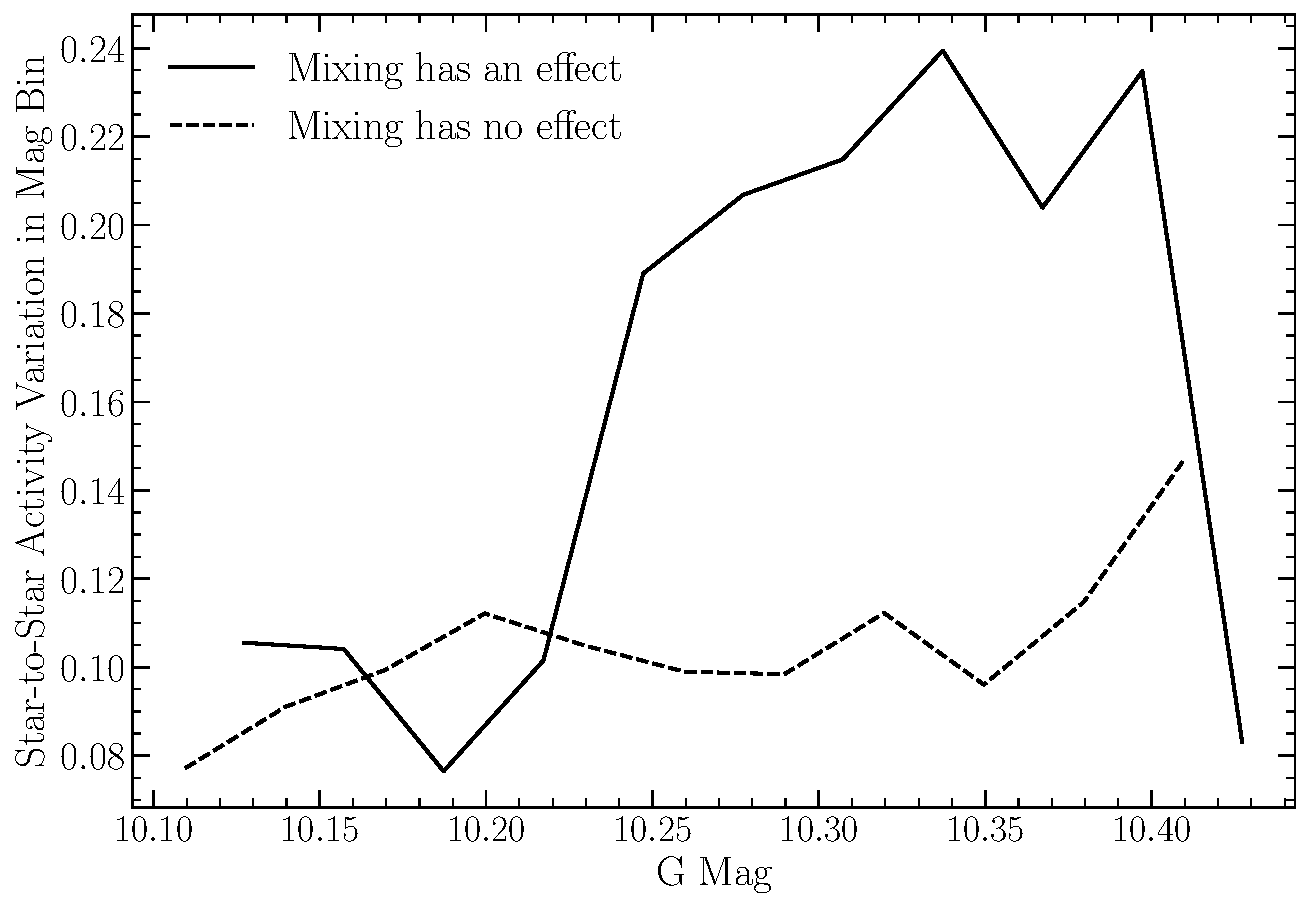
\includegraphics[width=0.85\textwidth]{figures/jaoMagActivity/SpreadModel.pdf}
  \caption{Toy model results showing a qualitatively similar discontinuity in the star-to-star magnetic activity variability.}
  \label{fig:model}
\end{figure}

\subsection{Limitations}
The model presented in this paper is very limited and it is important to keep
these limitations in mind when interpreting the results presented here. Some of
the main challenges which should be leveled at this model are the assumption
that the magnetic field will be altered by some small random perturbation at
every mixing event. This assumption was informed by the large number of free
parameters available to a physical star during the establishment of a large
scale magnetic field and the associated likely stochastic nature of that
process. However, it is similarly believable that the magnetic field will tend
to alter in a uniform manner at each mixing event. For example, since
differential rotation is generally proportional to the temperature gradient
within a star and activity is strongly coupled to differential rotation then it
may be that as the radiative zone reforms over thermal timescales the
homogenization of angular momentum throughout the star results in overall lower
amounts of differential rotation each after mixing event than would otherwise
be present.

Moreover, this model does not consider how other degenerate sources of magnetic
evolution such as stellar spin down, relaxation, or coronal heating may effect
star-to-star variability. These could conceivably lead to a similar increase in
star-to-star variability which is coincident with the Jao Gap magnitude as the
switch from fully to partially convective may effect efficiency of these
process.

Additionally, there are challenges with this toy model that originate from the
stellar evolutionary model. Observations of the Jao Gap show that the feature
is not perpendicular to the magnitude axis; rather, it is inversely
proportional to the color. No models of the Jao Gap published at the time of
writing capture this color dependency and \textit{what causes this color
dependency} remains one of the most pressing questions relating to the
underlying physics. This non captured physics is one potential explanation for
why the magnitude where our model predicts the increase in variability is not
in agreement with where the variability jump exists in the data.

Finally, we have not considered detailed descriptions of the dynamos of stars.
The magneto-hydrodynamical modeling which would be required to model the
evolution of the magnetic field of these stars at thermal timescale resolutions
over gigayears is currently beyond the ability of practical computing.
Therefore future work should focus on limited modeling which may inform the
evolution of the magnetic field directly around the time of a mixing event.

\section{Chemical Consistency}\label{sec:const}
There are three primary areas in which must the stellar models must be made
chemically consistent: the atmospheric boundary conditions, the opacities, and
interior abundances. The interior abundances are relatively easily handled by
adjusting parameters within our stellar evolutionary code. However, the other
two areas are more complicated to bring into consistency. Atmospheric boundary
conditions and opacities must both be calculated with a consistent set of
chemical abundances outside of the stellar evolution code.
{\bf Nearly all prior efforts at modeling multiple stellar populations in
globular clusters have adjusted the abundances used in the atmospheric interior
models, and in the high temperature opacities, but have not self-consistently
modified the corrosponding low-temperature opacities and surface bounary
conditions, as these are found from stellar atmosphere codes, and not the
stellar interior codes which are used to create stellar models and isochrones.
In this work, as in Dotter (2016), the stellar interior models are chemically
self-consistent with the stellar atmosphere models.} For evolution we The Dartmouth Stellar
Evolution Program (DSEP) \citep{Dotter2008}, a well tested 1D stellar evolution
code which has a particular focus on modelling low mass stars ($\le 2$
M$_{\odot}$)

\subsection{Atmospheric Boundary Conditions}\label{sec:atm}
Certain assumptions, primarily that the radiation field is at equilibrium and
radiative transport is diffusive \citep{Salaris2005}, made in stellar structure
codes, such as DSEP, are valid when the optical depth of a star is large.
However, in the atmospheres of stars, the number density of particles drops low
enough and the optical depth consequently becomes small enough that these
assumptions break down, and separate, more physically motivated, plasma
modeling code is required. Generally structure code will use tabulated
atmospheric boundary conditions generated by these specialized codes, such as ATLAS9
\citep{Kurucz1993}, PHOENIX \citep{Husser2013}, MARCS \citep{Gustafsson2008},
and MPS-ATLAS \citep{Kostogryz2023}. Often, as the boundary conditions are
expensive to compute, they are not updated as interior abundances vary. 

One key element when chemically consistently modeling NGC 2808 modeling is the
incorporation of new atmospheric models with the same elemental abundances as
the structure code. We use atmospheres generated from the \texttt{MARCS} grid
of model atmospheres \citep{Plez2008}. \texttt{MARCS} provides one-dimensional,
hydrostatic, plane-parallel and spherical LTE atmospheric models
\citep{Gustafsson2008}. Model atmospheres are made to match the
spectroscopically measured elemental abundances of populations A and E.
Moreover, for each population, atmospheres with various helium mass fractions
are generated. These range from Y=0.24 to Y=0.36 in steps of 0.03. All
atmospheric models are computed to an optical depth of $\tau = 100$ where their
temperature and pressures serves as boundary conditions for the structure code.
In general, enhancing helium in the atmosphere has only a small impact on the atmospheric
temperature profile, while leading to a drop in the pressure by $\sim 10 - 20 \%$.

\subsection{Opacities}\label{sec:opac}
In addition to the atmospheric boundary conditions, both the high and low
temperature opacities used by DSEP must be made chemically consistent. Here we
use OPLIB high temperature opacity tables \citep{Colgan2016} retrieved using
the TOPS web-interface. Retrival of High termperature opacities is done using
\texttt{pyTOPSScrape}, first introduced in \citet{Boudreaux2023}. Low
temperature opacity tables are retrieved from the Aesopus 2.0 web-interface
\citep{Marigo2009, Marigo2022}. Ideally, these opacities would be the same used
in the atmospheric models. However, the opacities used in the MARCS models are
not publicly available. As such, we use the opacities provided by the TOPS and
Aesopus 2.0 web-interfaces.

\section{fidanka}\label{sec:fidanka}
When fitting isochrones to the clusters with multiple populations we have four
main criteria for any method

\begin{itemize}
  \item The method must be robust enough to work along the entire main
    sequence, turn off, and much of the subgiant and red giant branch.
	\item Any method should consider photometric uncertainty in the fitting process.
	\item The method should be model independent, weighting any n number of populations equally.
	\item The method should be automated and require minimal intervention from the user.
\end{itemize}


We do not believe that any currently available software is a match for
our use case. Therefore, we elect to develop our own software suite, \fidanka.
\fidanka is a python package designed to automate much of the process of
measuring fiducial lines in CMDs, adhering to the four criteria we lay out
above. Primary features of \fidanka may be separated into three
categories: fiducial line measurement, stellar population synthesis, and
isochrone optimization/fitting. Additionally, there are utility functions that
are detailed in the \fidanka documentation.

\subsection{Fiducial Line Measurement}
\fidanka takes a iterative approach to measuring fiducial lines, the first step
of which is to make a ``guess'' as to the fiducial line. This initial guess
is calculated by splitting the CMD into magnitude bins, with uniform numbers of
stars per bin (so that bins are cover a small magnitude range over densely
populated regions of the CMD while covering a much larger magnitude range in
sparsely populated regions of the CMD, such as the RGB). A unimodal Gaussian
distribution is then fit to the color distribution of each bin, and the
resulting mean color is used as the initial fiducial line guess. This rough
fiducial line will approximately trace the area of highest density. The initial
guess will be used to verticalze the CMD so that further algorithms can work in
1-D magnitude bins without worrying about weighting issues caused by varying
projections of the evolutionary sequence onto the magnitude axis.
Verticalization is preformed taking the difference between the guess fiducial
line and the color of each star in the CMD.

If \fidanka were to simply apply the same algorithm to the verticalized CMD
then the resulting fiducial line would likely be a re-extraction of the initial
fiducial line guess. To avoid this, we take a more robust, number density based
approach, which considers the distribution of stars in both color and magnitude
space simultaneously. For each star in the CMD we first use an
\texttt{introselect} partitioning algorithm to select the 50 nearest stars in
F814W vs. F275W-F814W space. To account for the case where the star is at an
extreme edge of the CMD, those 50 stars include the star itself (such that we
really select 49 stars + 1). We use
\texttt{qhull}\footnote{https://www.qhull.com}\citep{Barber1996} to calculate
the convex hull of those 50 points. The number density at each star then is
defined as $50/A_{hull}$, where $A_{hull}$ is the area of the convex hull.
Because we use a fixed number of points per star, and a partitioning algorithm
as opposed to a sorting algorithm, this method scales like $\mathcal{O}(n)$,
where n is the number of stars in the CMD. This method also intrinsically
weights the density of of each star equally as the counting statistics per bin
are uniform. We are left with a CMD where each star has a defined number
density (Figure \ref{densityMapDemo}).

\begin{figure*}
	\centering
	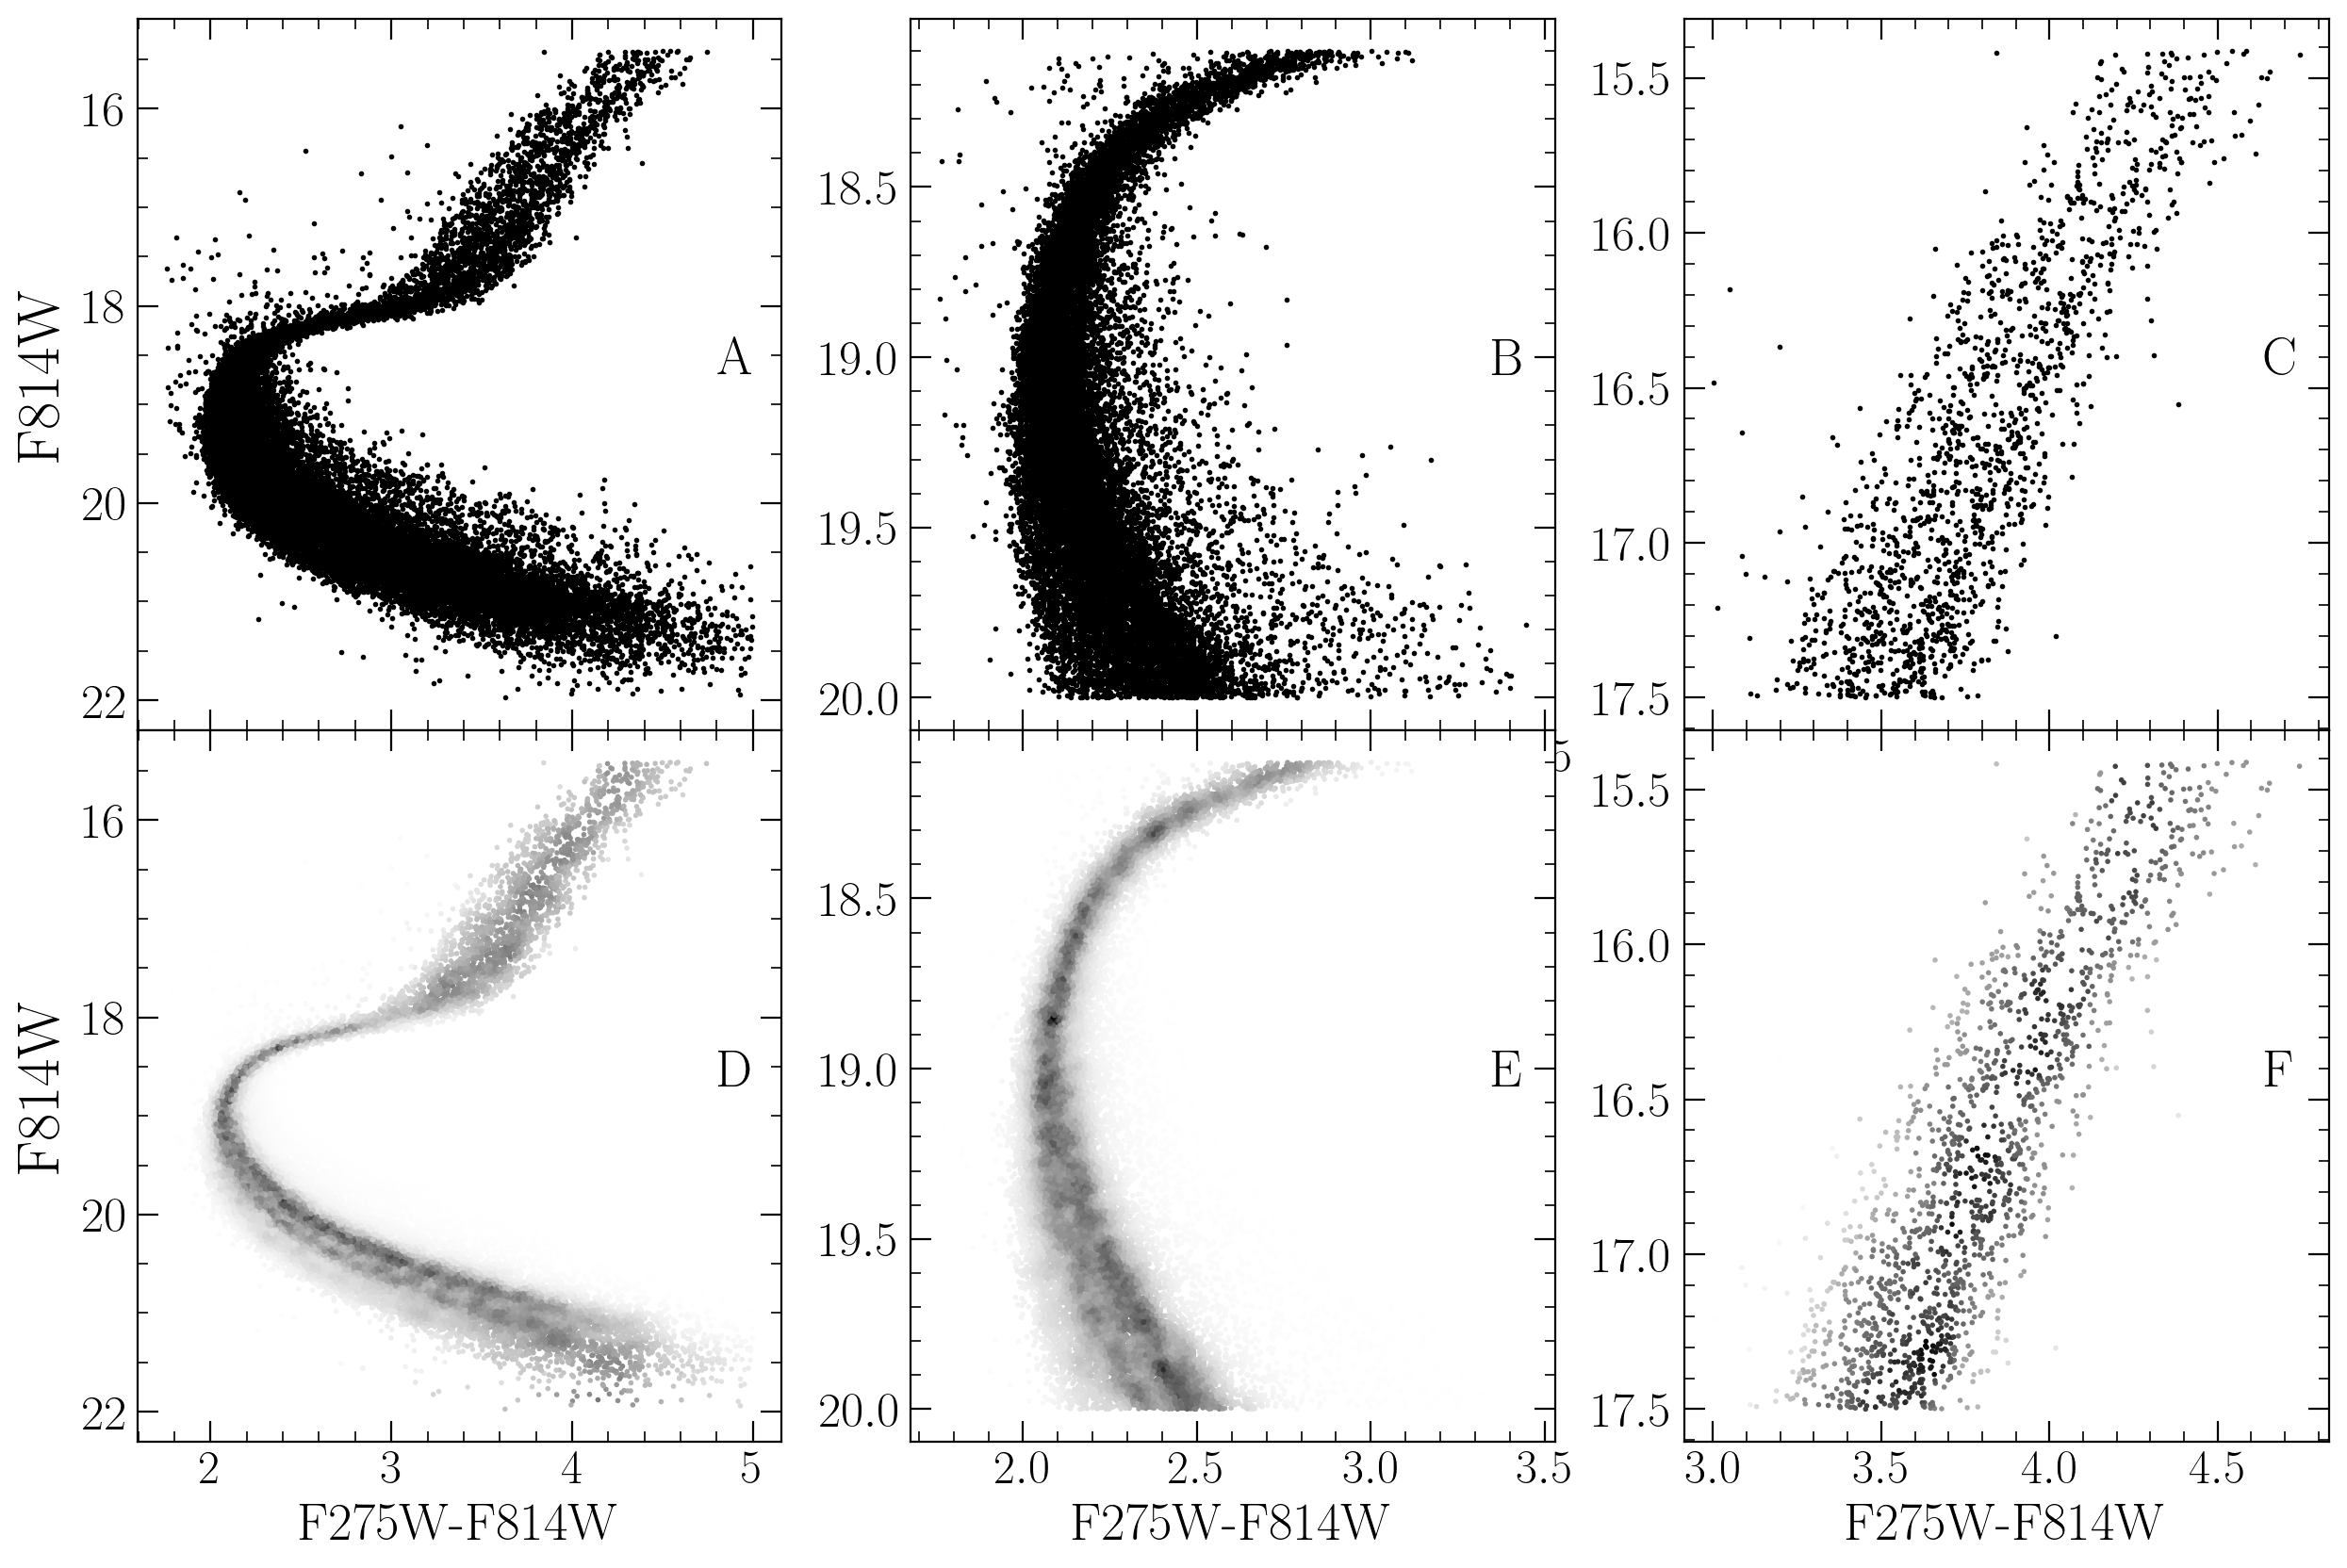
\includegraphics[width=0.9\textwidth]{figures/ngc2808/notebookFigures/DensityMapDemo.png}
  \caption{Figures in the top row are the raw CMD, while figures in the bottom
  row are colored by the density map.Density map demo showing density estimate
  over different parts of the evolutionary sequence. The left panel shows the
  density map over the entire evolutionary sequence, while the middle panel
  shows the density map over the main sequence and the right most panel shows
  the density map over the RGB. }
	\label{densityMapDemo}
\end{figure*}

\fidanka can now exploit this density map to fit a better fiducial line to the
data, as the density map is far more robust to outliers. There are multiple
algorithms we implement to fit the fiducial line to the color-density profile
in each magnitude bin (Figure \ref{densityBinsDemo}); they are explained in
more detail in the \fidanka documentation. However, of most relevance here is
the Bayesian Gaussian Mixture Modeling (BGMM) method. BGMM is a clustering
algorithm which, for some fixed number of n-dimensional Gaussian distributions,
$K$, determines the mean, covariance, and mixing probability (somewhat
analogous to amplitude) of each $k^{th}$ distribution, such that the local
lower bound of the likelyhood of each star belonging strongly to a single
distribution is maximized. 

\begin{figure}
	\centering
	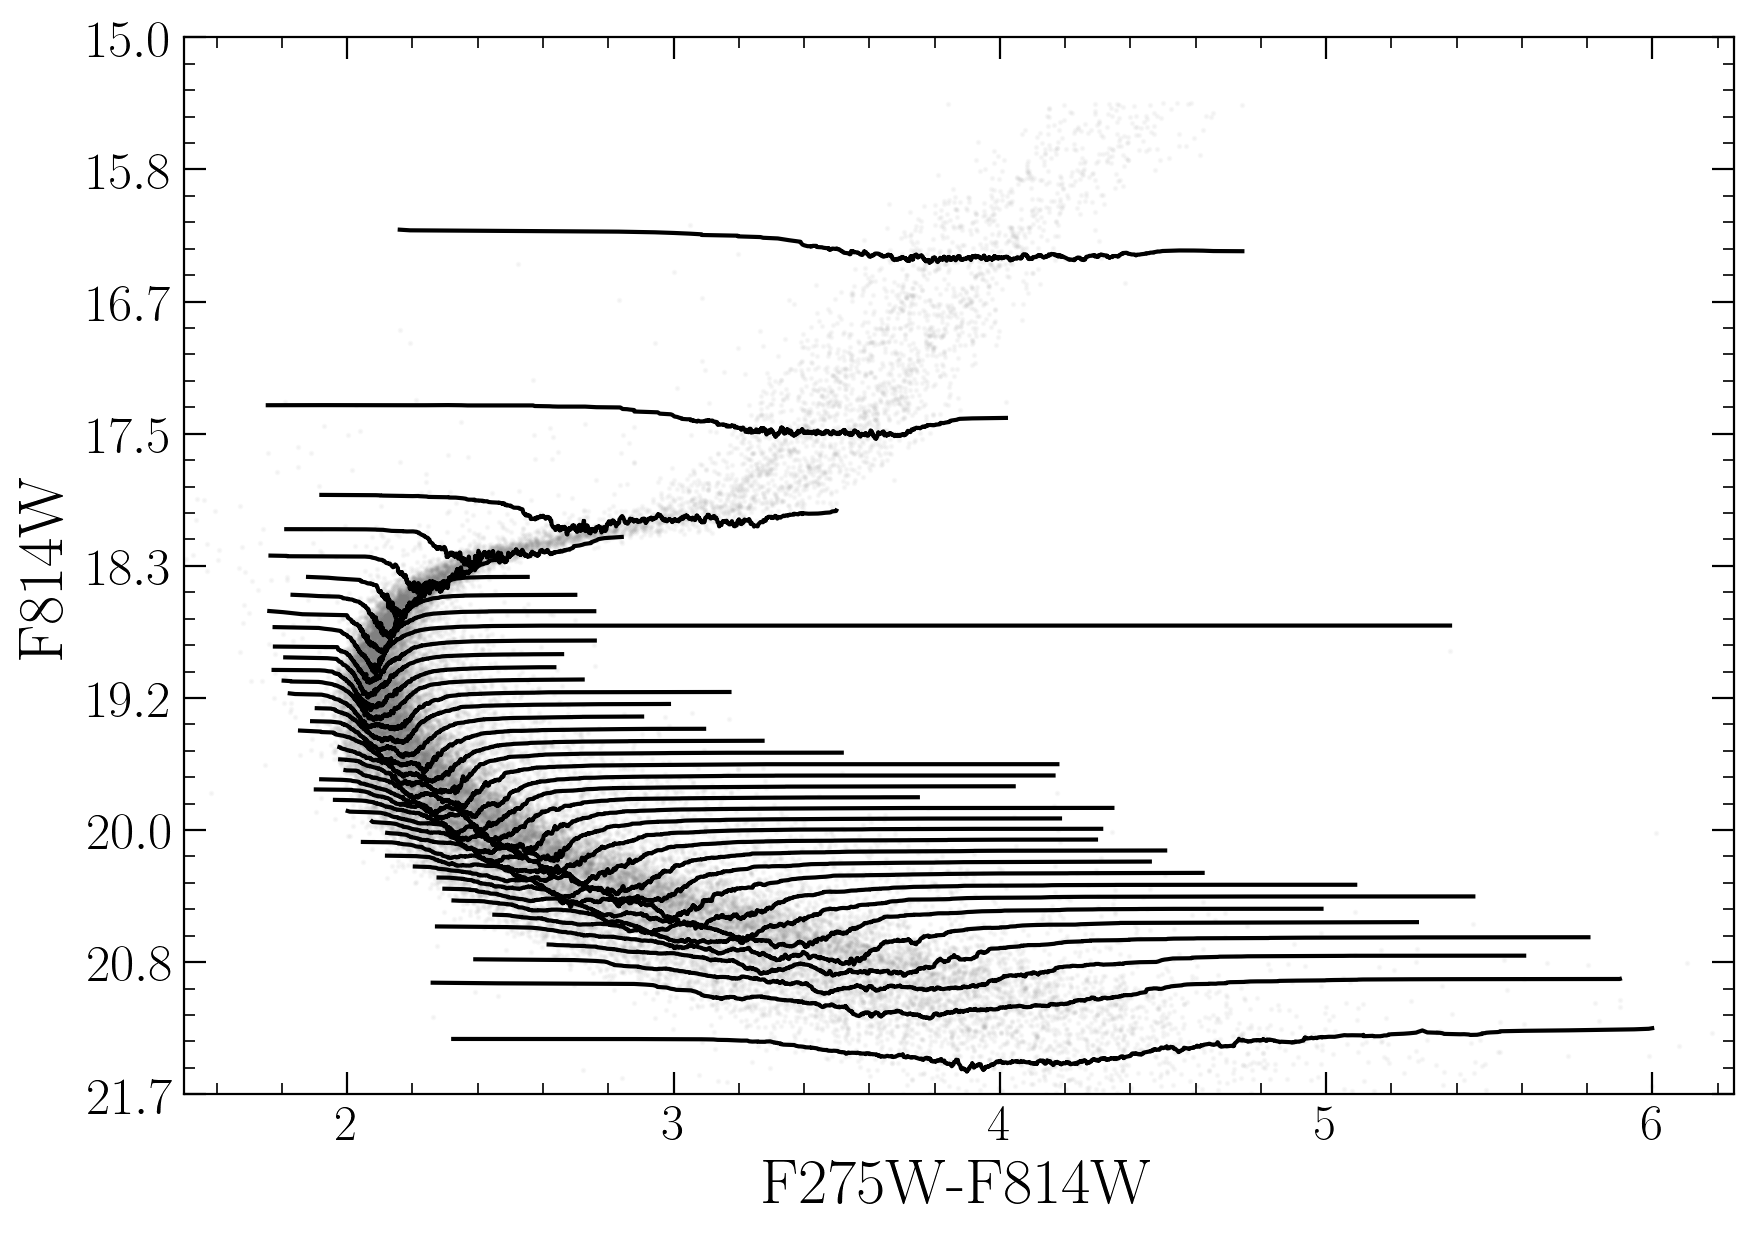
\includegraphics[width=0.85\textwidth]{figures/ngc2808/notebookFigures/DensityBinsDemo.png}
	\caption{CMD where point brightness is determined by local density. Lines show the
	density-color profile in each magnitude bin. In this figure adaptive
	binning targeted 1000 stars per bin}
	\label{densityBinsDemo}
\end{figure}

Maximization is preformed using the Dirichlet process, which is a
non-parametric Bayesian method of determining the number of Gaussian
distributions, $K$, which best fit the data \citep{Ferguson1973, scikit-learn}.
Use of the Dirichlet process allows for dynamic variation in the number of
inferred populations from magnitude bin to magnitude bin. Specifically,
populations are clearly visually separated from the lower main sequence through
the turn off; however, at the turn off and throughout much of the subgiant
branch, the two visible populations overlap due to their extremely similar ages
\citep[i.e.][]{Jordan2002}. The Dirichlet process allows for the BGMM method to
infer a single population in these regions, while inferring two populations in
regions where they are clearly separated. More generally, the use of the
Dirichlet process removes the need for a prior on the exact number of
populations to fit. Rather, the user specifies a upper bound on the number of
populations within the cluster. An example bin (F814W = 20.6) is shown in
Figure \ref{fig:BGMMDist}.

\begin{figure*}
	\centering
	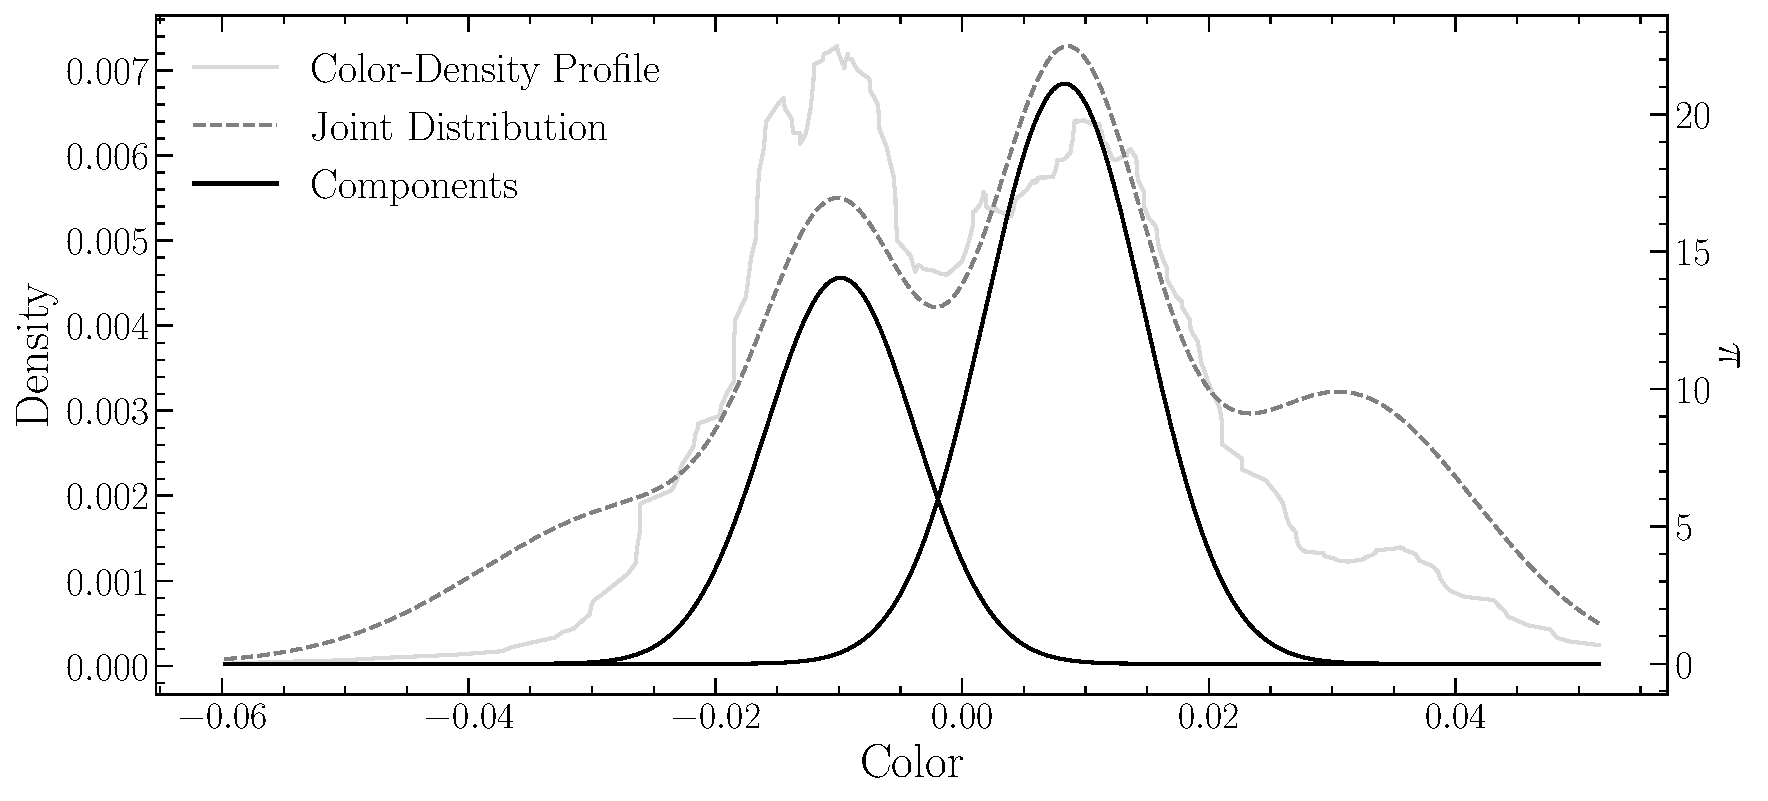
\includegraphics[width=0.9\textwidth]{figures/ngc2808/BGMMMixingBin.pdf}
	\caption{Example of BGMM fit to a magnitude bin. The grey line shows the
	underlying color-density profile, while the black dashed-line shows the
	joint distribution of each BGMM component. The solid black lines show the
	two selected components.}
	\label{fig:BGMMDist}
\end{figure*}

\fidanka's BGMM method first breaks down the verticalized CMD into magnitude
bins with uniform numbers of stars per bin (here we adopt 250). Any stars left
over are placed into the final bin. For each bin a BGMM model with a maximum of
5 populations is fit to the color density profile. The number of populations is
then inferred from the weighting parameter (the mixing probability) of each
population. If the weighting parameter of any $k^{th}$ components less than
{\color{blue}0.05}, then that component is considered to be spurious and
removed. Additionally, if the number of populations in the bin above and the
bin below are the same, then the number of populations in the current bin is
forced to be the same as the number of populations in the bin above. Finally,
the initial guess fiducial line is added back to the BGMM inferred line. Figure
\ref{fig:vertFit} shows the resulting fiducial line(s) in each magnitude bin
for both a verticalized CMD and a non verticalized CMD. In contrast to other
work in the literature where evidence for up to 5 distinct populations has been
found; we only find evidence for two stellar populations.

\begin{figure}
	\centering
	\includegraphics[width=0.65\textwidth]{figures/ngc2808/vertFit.png}
  \caption{Verticalized CMD (where the color of each data point is subtracted
  from the color of the fiducial line at that magnitude) where point brightness
  is determined by density (top). CMD where point brightness is determined by
  density, calculated fiducial lines are shown (bottom). The data used is from
  the Hubble Space Telescope UV Legacy Survey of Galactic Globular Clusters.}
	\label{fig:vertFit}
\end{figure}

This method of fiducial line extraction effectively discriminated between
multiple populations along the main sequence and RGB of a cluster, while
simultaneously allowing for the presence of a single population along the MSTO
and subgiant branch. 

We can adapt this density map based BGMM method to consider photometric
uncertainties by adopting a simple Monte Carlo approach. Instead of measuring
the fiducial line(s) a single time, \fidanka can measure the fiducial line(s)
many times, resampling the data with replacement each time. For each resampling
\fidanka adds a random offset to each filter based on the photometric
uncertainties of each star. From these $n$ measurements the mean fiducial line
for each sequence can be identified along with upper and lower bound confidence
intervals in each magnitude bin.

\subsection{Stellar Population Synthesis}
While not extensively used in this paper \fidanka can, in addition to measuring fiducial
lines, preform stellar population synthesise. \fidanka's population synthesis
module can generate synthetic stellar population from a set of MIST formatted
isochrones. This is of primary importance for binary population modeling. The
module is also used to generate synthetic CMDs for the purpose of testing the
fiducial line extraction algorithms against priors.

\fidanka uses MIST formatted isochrones \citep{Dotter2016} as input along
with distance modulus, B-V color excess, binary mass fraction, and bolometric
corrections. An arbitrarily large number of isochrones may be used to define an
arbitrary number of populations. Synthetic stars are samples from each
isochrone based on a definable probability (for example it is believed that
$\sim90\%$ of stars in globular clusters are younger population
\citep[e.g.][]{Suntzeff1996, Carretta2013}). Based on the metallicity, $\mu$, and E(B-V) of each
isochrone, bolometric corrections are taken from bolometric correction tables.
Where bolometric correction tables do not include exact metallicities or
extinctions a linear interpolation is preformed between the two bounding
values. 

\subsection{Isochrone Optimization}
The optimization routines in \fidanka will find the best fit distance modulus,
B-V color excess, and binary number fraction for a given set of isochrones. If
a single isochrone is provided then the optimization is done by minimizing the
$\chi^2$ of the perpendicular distances between an isochrone and a fiducial
line. If multiple isochrones are provided then those isochrones are first used
to run stellar population synthesis and generate a synthetic CMD. The
optimization is then done by minimizing the $\chi^2$ of both the perpendicular
distances between and widths of the observed fiducial line and the fiducial
line of the synthetic CMD.


\subsection{Fidanka Testing}
In order to validate fidanka we have run an series of injection recovery tests
using \fidanka's population synthesis routines to build various synthetic
populations and \fidanka's fiducial measurement routines to recover these
populations. Each population was generated using the initial mass function
given in \citep{Milone2012} for the redmost population ($\alpha=-1.2$).
Further, every population was given a binary population fraction of 10\%,
distance uniformly sampled between 5000pc and 15000pc, and a B-V color excess
uniformly sampled between 0 and 0.1. Finally, each synthetic population was
generated using a fixed age  uniformlly sampled between 7 Gyr and 14 Gyr. An
example synthetic population along with its associated best fit isochrone are
shown in Figure \ref{fig:ValidationBestFit}.

\begin{figure}
  \centering
  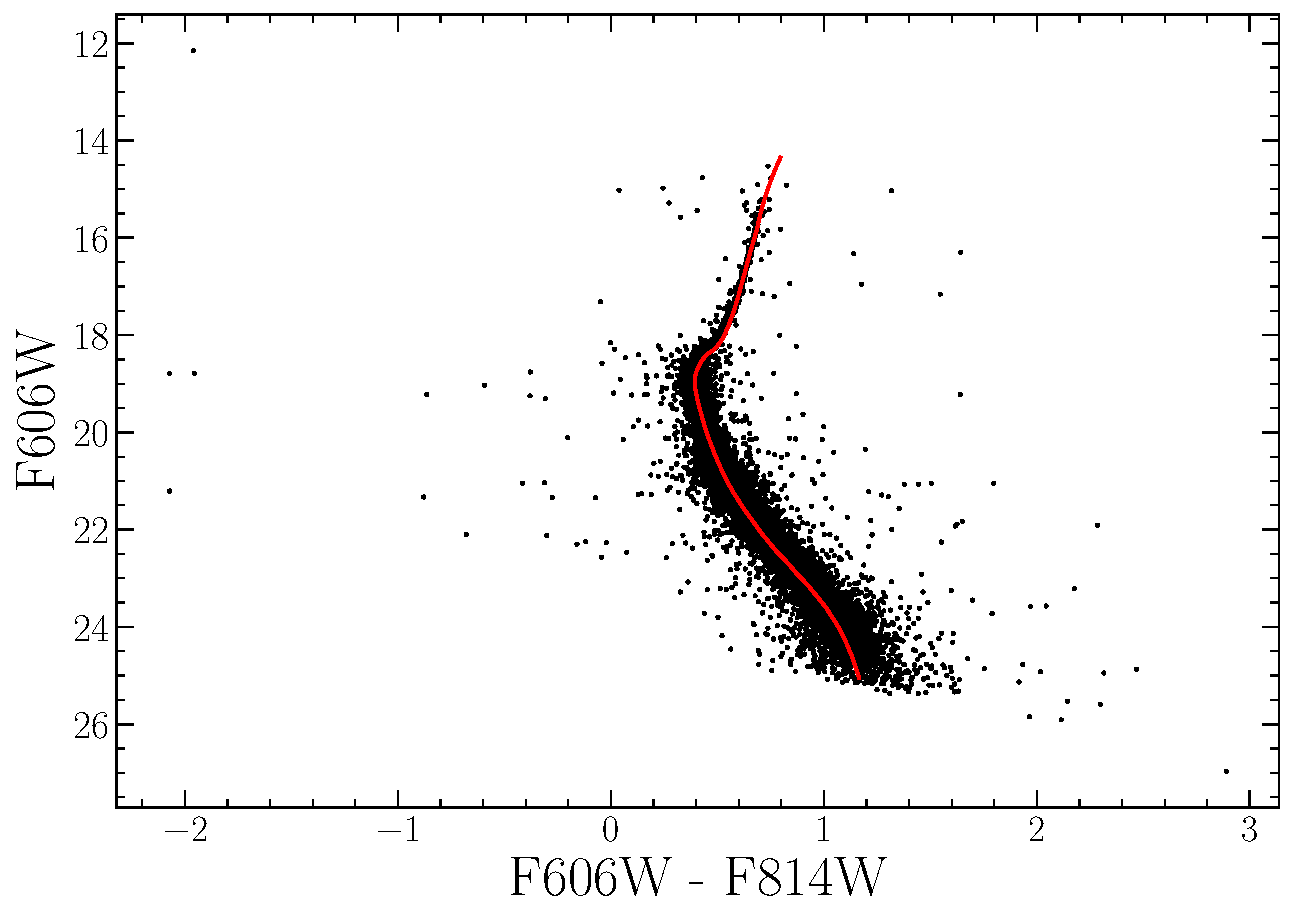
\includegraphics[width=0.85\textwidth]{figures/ngc2808/ExtractedIsoFit.pdf}
  \caption{Synthetic population generated by fidanka at 10000pc with E(B-V) =
  0, and an age of 12 Gyr along with the best fitting isochrone. The best fit
  paremeters are derived to be $mu=15.13$, E(B-V)=0.001, and an age of 12.33
  Gyr.}
  \label{fig:ValidationBestFit}
\end{figure}

For each trial we use \fidanka to measure the fiducial line and then optimize
that fiducial line against the originating isochrone to esimate distance
modulus, age, and color B-V excess. Figure \ref{fig:validationDist} is built
from 1000 Monte-Carlo trials and shows the mean and width of the percent
error distributions for $\mu$, $A_{v}$, and age. In general \fidanka is able to
recover distance modulii effectively with age and E(B-V) reovery falling in
line with other literature that does not cosider the CMD outside of the main
sequence, main sequence turn off, sub giant, and red giant branches;
specifically, it should be noted that \fidanka is not setup to model the
horizontal branch.

\begin{figure}
  \centering
  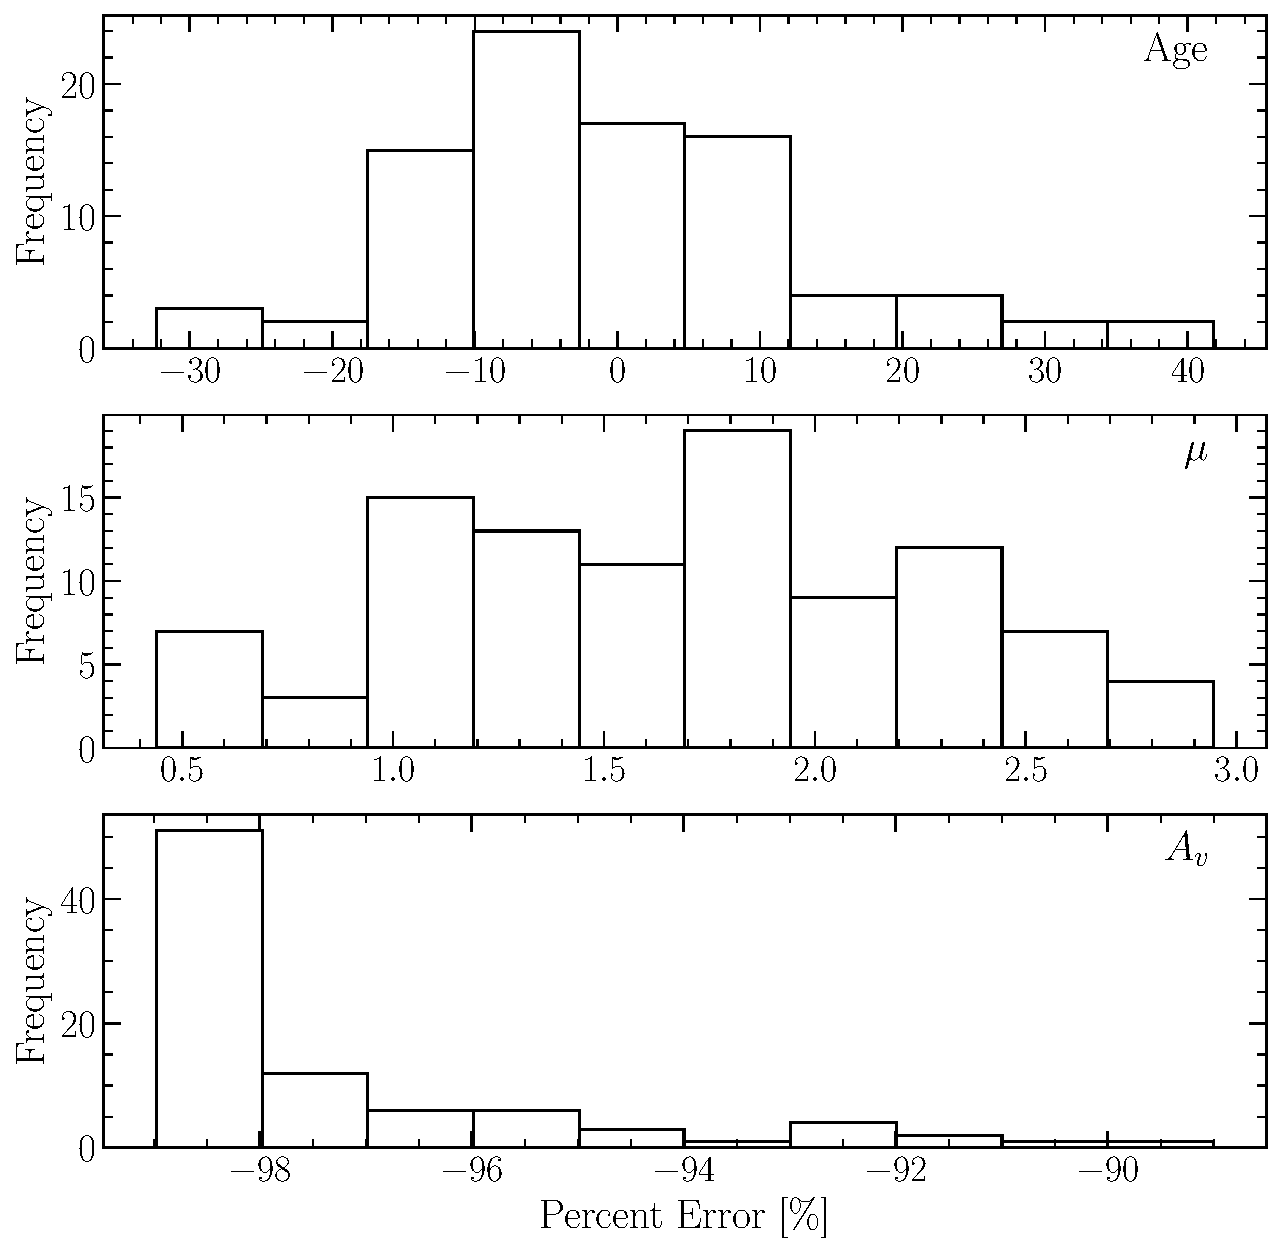
\includegraphics[width=0.85\textwidth]{figures/ngc2808/DistributionOfErrors.pdf}
  \caption{Percent Error distribution for each of the three deriver parameters.
  Note that these values will be sensitive to the magnitude uncertainties of
  the photometry. Here we made use of the ACS artificial star tests to estimate
  the uncertanties.}
  \label{fig:validationDist}
\end{figure}

\section{Isochrone Fitting}\label{sec:isoFit}
We fit pairs of isochrones to the HUGS data for NGC 2808 using \fidanka, as
descrbed in \S \ref{sec:fidanka}. Two isochrones, one for Population
A and one for Population E are fit simultaneously. These isochrones are
constrained to have distance modulus, $\mu$, and color excess, E(B-V) which
agree to within 1\%. Moreover, we constrain the mixing length, $\alpha_{ML}$, for any two isochrones in a set to be within 0.5 of one and other. For every isochrone in the
set of combination of which fulfilling these constraints $\mu$, $E(B-V)$,
Age$_{A}$, and $Age_{B}$ are optimized to reduce the $\chi^{2}$ distance
between the fiducial lines and the isochrones. Because we fit fiducial lines
directly, we do not need to consider the binary population fraction, $f_{bin}$,
as a free parameter.

The best fit isochrones are shown in Figure \ref{fig:BestFitResults} and optimized
parameters for these are presented in Table \ref{tab:BestFitResults}. We find helium mas fractions which are consistent with those identified in past literature \citep[e.g.][]{Milone2015}. Note that our helium mass fraction gird has a spacing of 0.03 between grid points and we are therefore unable to resolve between certain proposed helium mass fractions for the younger sequence (for example between 0.37 and 0.39).

\begin{figure*}
  \centering
  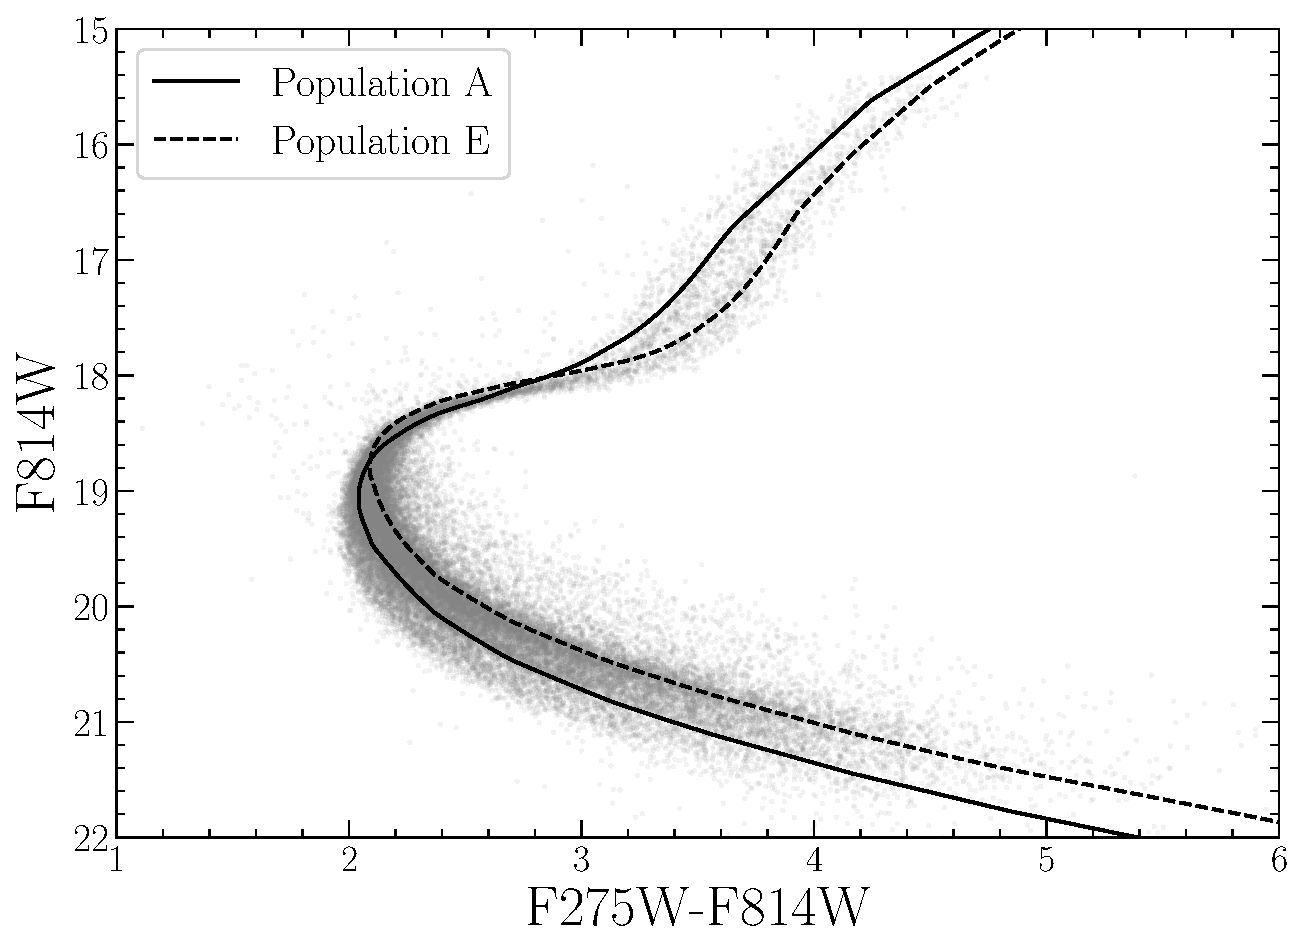
\includegraphics[width=0.9\textwidth]{figures/ngc2808/BestFitResults.pdf}
  \label{fig:BestFitResults}
  \caption{Best fit isochrone results for NGC 2808.}
\end{figure*}

\begin{table*}
  \centering
  \begin{tabular}{c | c c c c c c}
    \hline
    population & age & distance modulus & extinction & Y & $\alpha_{ML}$ & $\chi^{2}_{\nu}$\\
    & [Gyr] & & [mag] & & &\\
    \hline
    \hline
    A & 12.3 & 14.91 & 0.54 & 0.24 & 1.901 & 0.014\\
    E & 14.3 & 14.96 & 0.54 & 0.39 & 1.750 & 0.017 \\
    \hline
  \end{tabular}
  \label{tab:BestFitResults}
  \caption{Best fit parameters derived from fitting isochrones to the fiducual lines derived from the NCG 2808 photometry.}
\end{table*}


Past literature \citep[e.g. ][]{Milone2015, Milone2018} have found helium mass fraction variation from the low redmost to bluemost populations of $\sim 0.12$. Here we find a helium mass fraction variation of 0.15 which, given the spacing of the helium grid we use \textbf{is consistent with these past results}.

\subsection{The Number of Populartions in NGC 2808}
In order to estimate the number of populations which ideally fit the NGC 2808
F275W-F814W photometry without overfitting the data we make use of silhouette
analysis \citep[][and in a similar manner to how \citet{Valle2022}
preform their analysis of spectroscopic data]{ROUSSEEUW198753}. We find the average silhouette score for all tagged
clusters identified using BGMM in all magnitude bins over the CMD using the
standar python module \texttt{sklearn}. Figure \ref{fig:clusterAn} shows the
silhouette analysis results and that 2 populations fit the photometry most
ideally. This is in line with what our BGMM model predicts for the majority of
the the CMD.

\begin{figure}
  \centering
  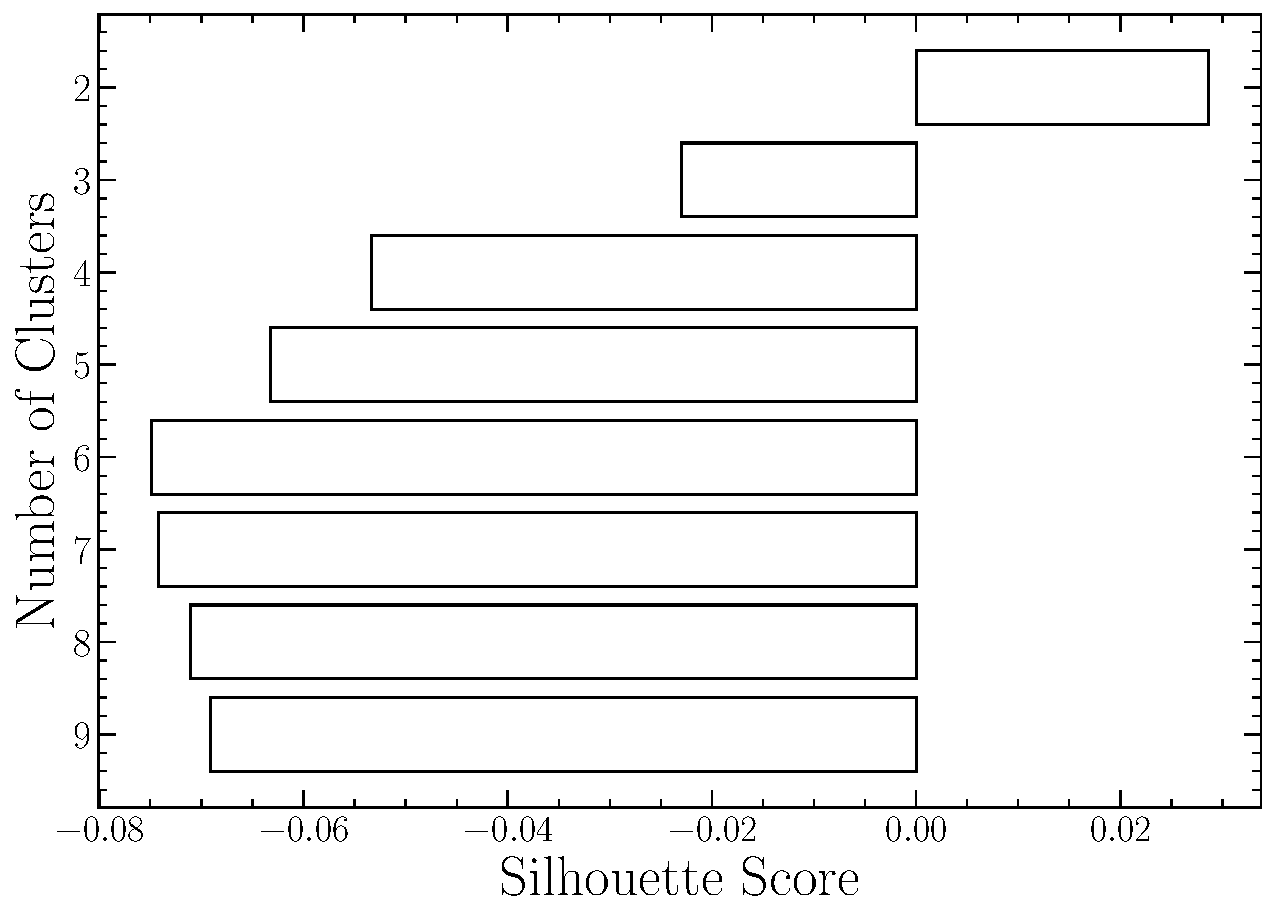
\includegraphics[width=0.45\textwidth]{figures/ngc2808/ClusterAnalysis.pdf}
  \caption{Silhouette analysis for NGC 2808 F275W-F814W photometry. The Silhouette scores
  are an average of score for each magnitude bin. Positive scores incidate that the clustering
  algorithm produced well distinguised clusters while negative scores indicate clusters which are not
  well distinguised.}
  \label{fig:clusterAn}
\end{figure}


\subsection{ACS-HUGS Photometric Zero Point Offset}
The Hubble legacy archive photometry used in this work is calibrated to the
Vega magnitude system. However, we have found that the photometry has a
systematic offset of $\sim0.026$ magnitudes in the F814W band when
compared to the same stars in the ACS survey (Figure \ref{fig:offset}). The
exact cause of this offset is unknown, but it is likely due to a difference in
the photometric zero point between the two surveys. A full correction of this
offset would require a careful re-reduction of the HUGS photometry, which is
beyond the scope of this work. We instead recognize a 0.02 inherent uncertainty
in the inferred magnitude of any fit when comparing to the ACS survey. This
uncertainty is small when compared to the uncertainty in the
distance modulus and should not affect the conclusion of this
paper. 

\begin{figure*}
  \centering
  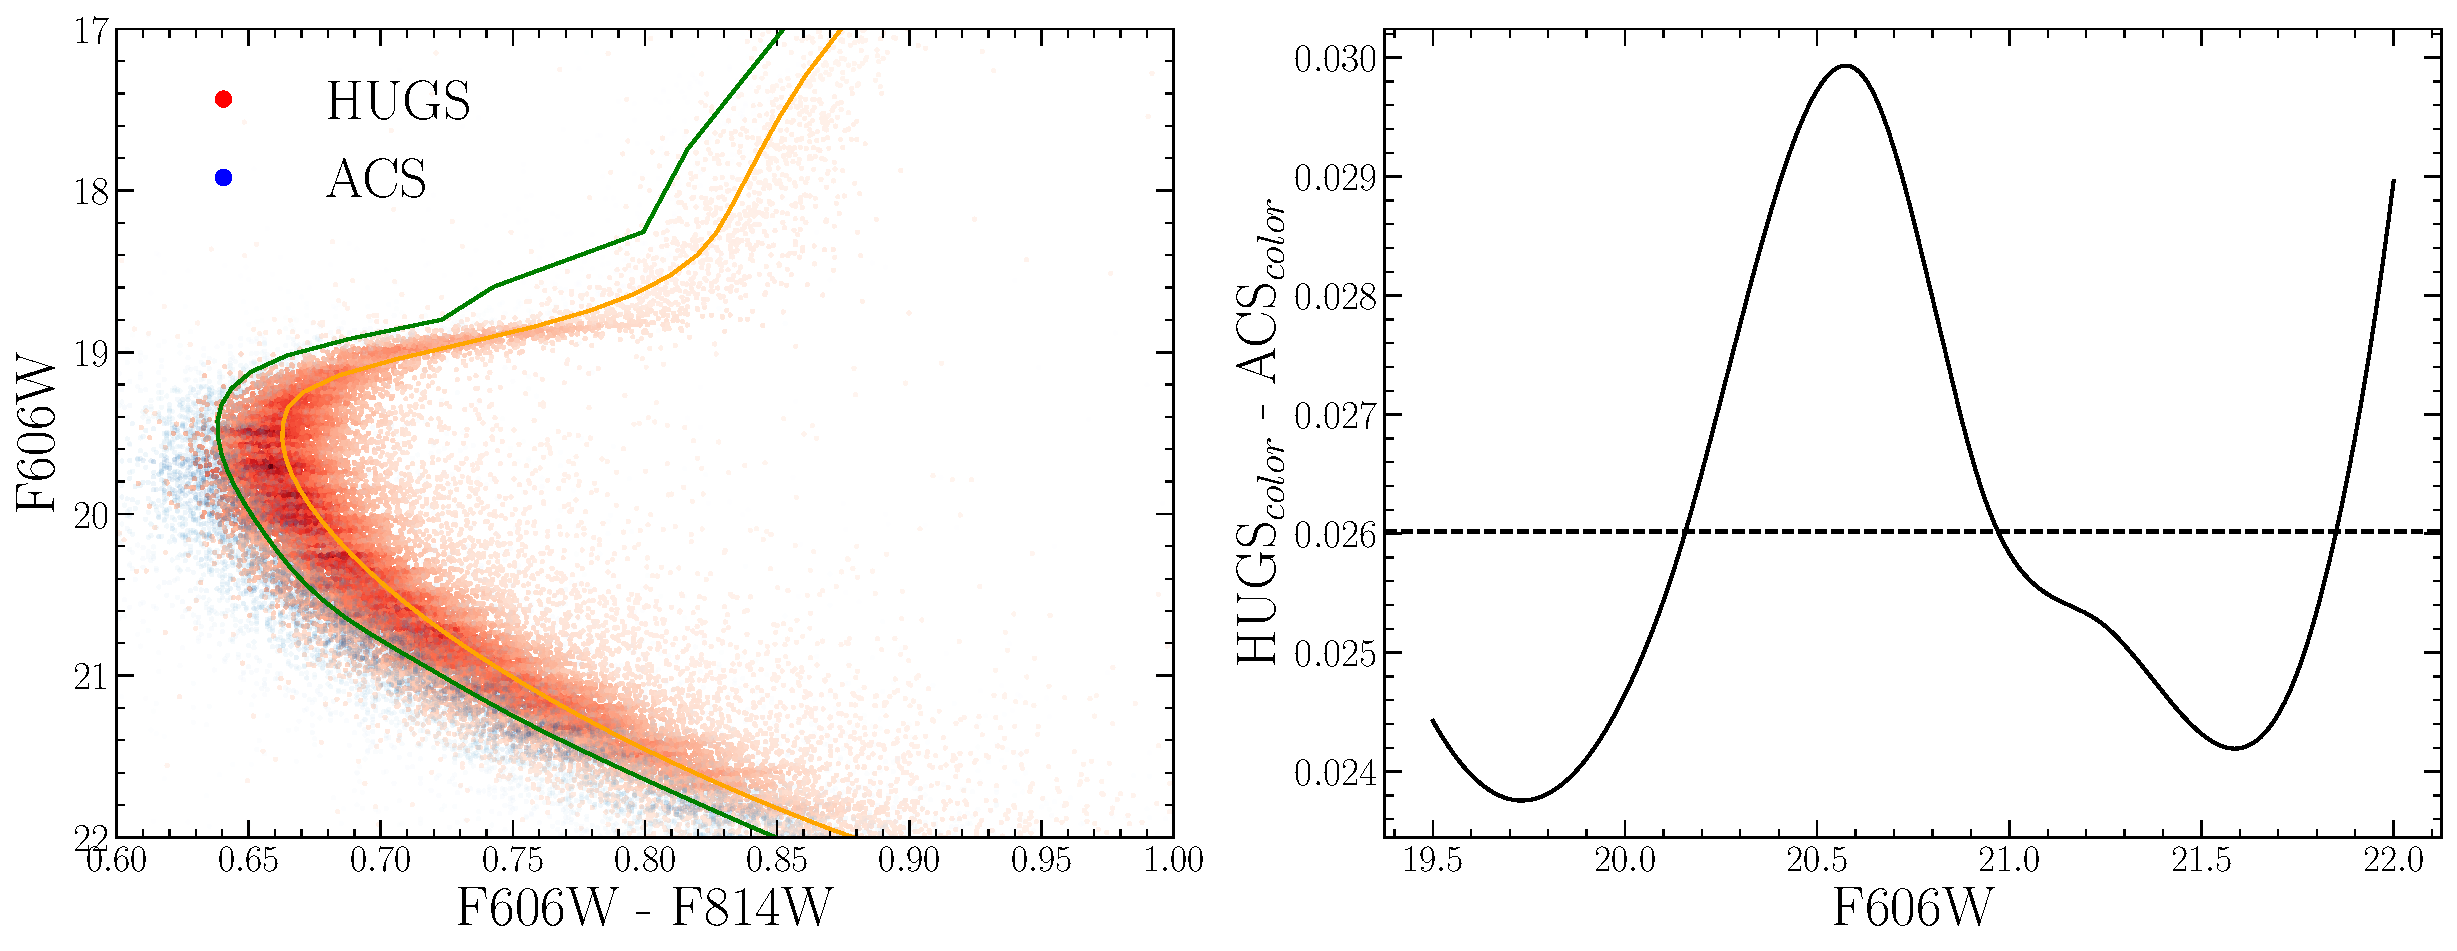
\includegraphics[width=0.90\textwidth]{figures/ngc2808/photometricOffset.pdf}
  \label{fig:offset}
  \caption{(left) CMD showing the photometric offset between the ACS and HUGS data for NGC 2808. CMDs have been randomly subsampled and colored by point density for clarity. (right) Mean difference between the color of the HUGS and ACS fiducual lines at the same magnitude. Note that the ACS data is systematically bluer than the HUGS data.}
\end{figure*}

The oberved photometric offset between ACS and HUGS reductions introduces a
systematic uncertainity when comparing parameters derived from isochrone fits
to ACS data vs those fit to HUGS data. Specifically, this offset introduces a
{\color{red}$\sim$AGE Gyr} uncertainity. Moreover, for two isochrone of the
same age, only seperated by helium mass fraction, a shift of the main sequence
turn off of is also expected. Figure \ref{fig:HeMO} shows this shift. Note a change in the helium mass fraction of a model by 0.03 results in an approximate 0.08 magnitude shift to the main sequence turn off location. This means that the mean 0.026 magnitude offset we find in between ACS and HUGS data corresponds to an additional approaximate 0.01 uncertainity in the derived helium mass fraction when comparing between these two datasets. 

\begin{figure}
  \centering
  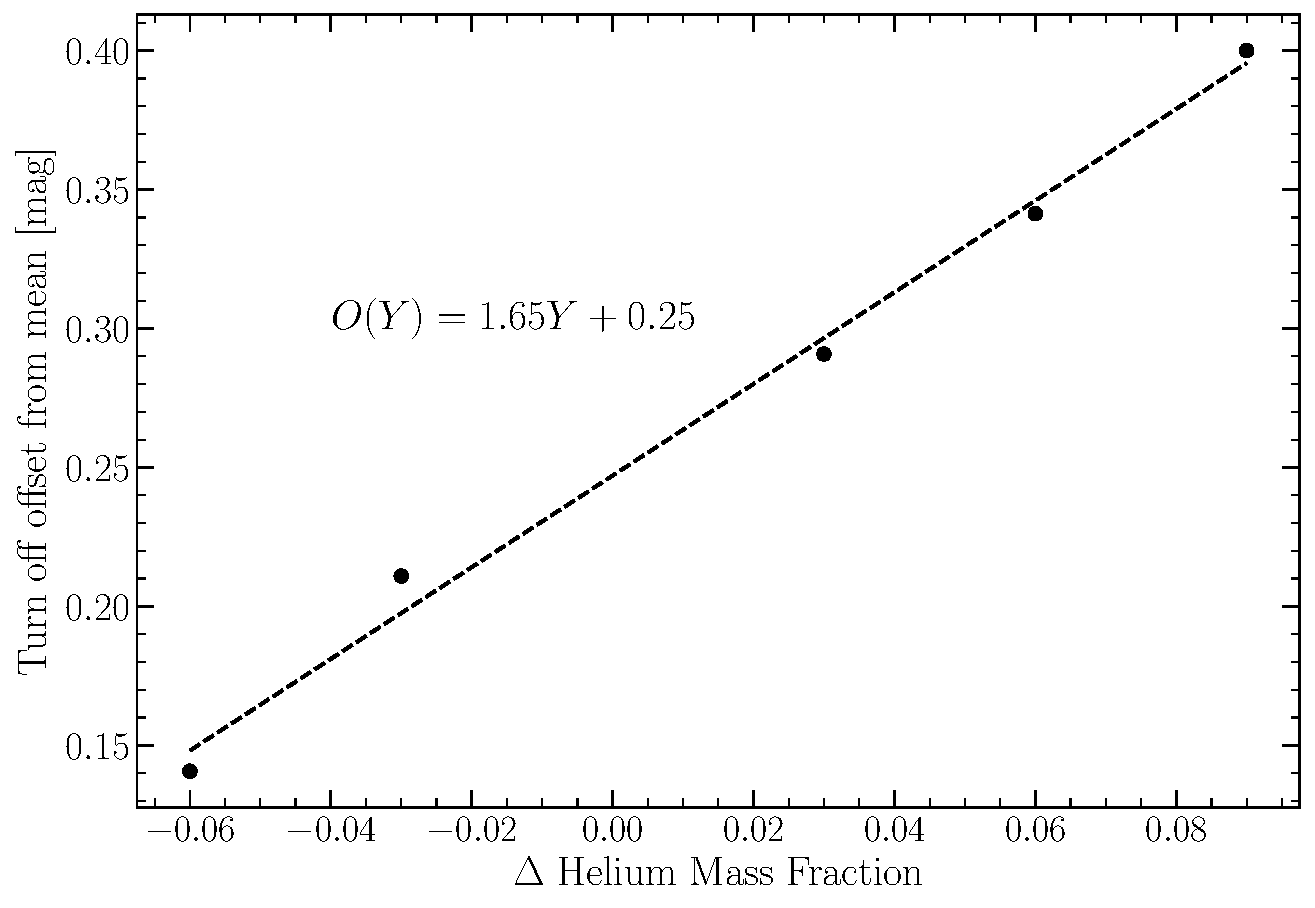
\includegraphics[width=0.45\textwidth]{figures/ngc2808/HeliumMeanOffset.pdf}
  \caption{Main sequence turn off magnitude offset from a guage helium mass fraction (Y=0.30 chosen). All main sequence turn off locations are measured at 12.3 Gyr {\color{blue} Should I make these contour surfaces for various ages?}}
  \label{fig:HeMO}
\end{figure}

\section{Correlation}\label{sec:results}
Using Ca II H\&K emission data from \citet{Boudreaux2022} and
\citet{Perdelwitz2021} (quantified using the $R_{HK}$ metric) we investigate
the correlation between the Jao Gap magnitude and stellar magnetic activity. We
are more statistically limited here than past authors have been due to
the requirement for high resolution spectroscopic data when measuring Calcium
emission; however, this is balanced by the apparent stronger correlation between
Calcium emission and the Jao gap when compared to H$\alpha$ emission. 

The merged dataset is presented in Figure \ref{fig:mergedData}. There is a
visual discontinuity just below the Jao Gap magnitude; however, this
manifests as an increase in the spread of the emission measurements rather than
a change in the mean value. In order to quantify the significance of this
discontinuity we measure the false alarm probability of the change in standard
deviation.

\begin{figure}
  \centering
  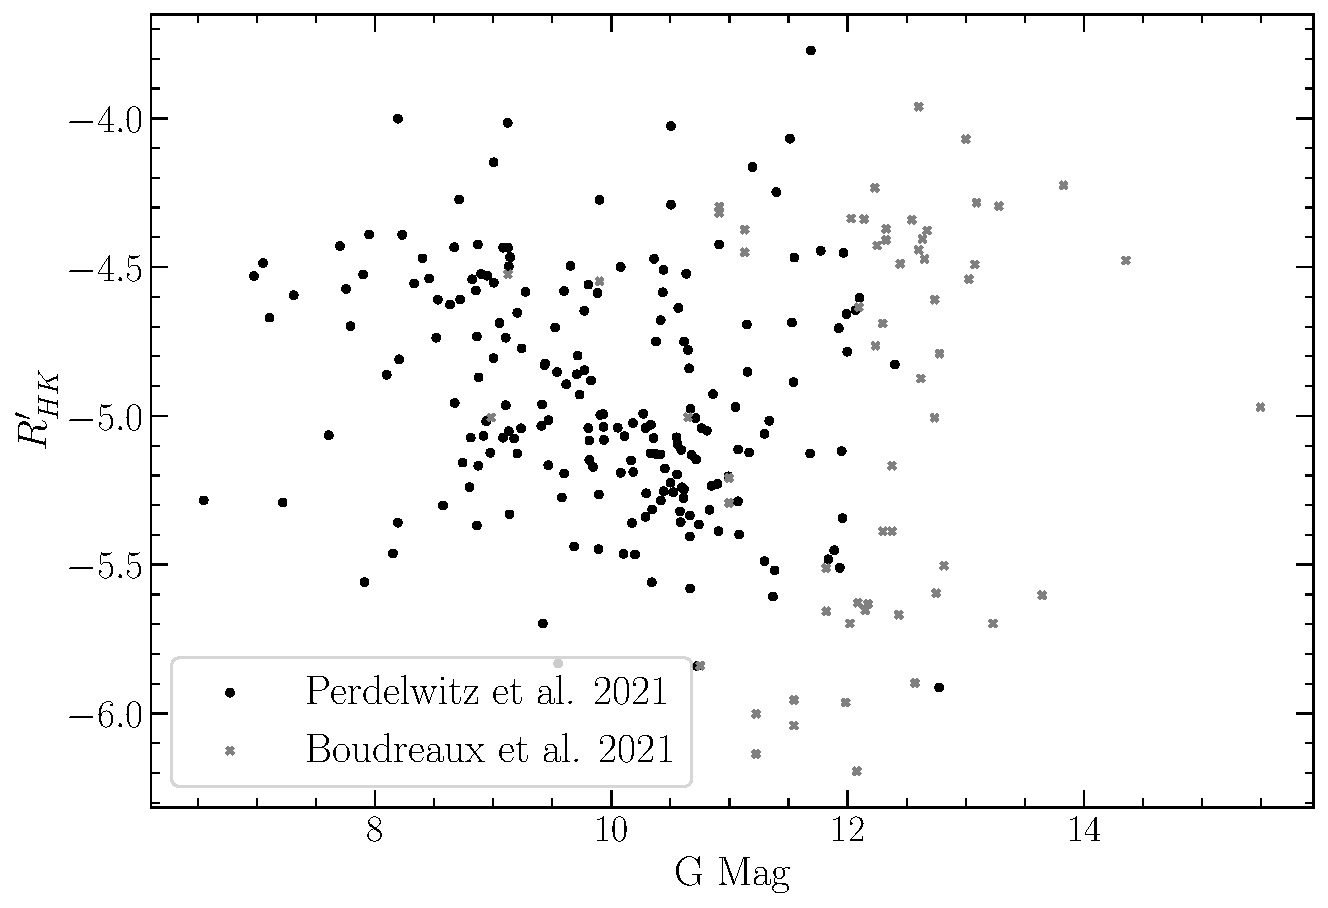
\includegraphics[width=0.45\textwidth]{figures/jaoMagActivity/Combined.pdf}
  \caption{Merged Dataset from \citet{Boudreaux2022, Perdelwitz2021}. Note the
  increase in the spread of $R'_{HK}$ around the Jao Gap Magnitude.}
  \label{fig:mergedData}
\end{figure}

First we split the merged dataset into bins with a width of 0.5 mag. In each bin we
measure the standard deviation about the mean of the data. The results of this
are shown in Figure \ref{fig:deviation}. In order to measure the false alarm
probability of this discontinuity we first resample the merged calcium
emission data based on the associated uncertainties for each datum as
presented in their respective publications. Then, for each of these ``resample
trials'' we measure the probability that a change in the standard deviation of
the size seen would happen purely due to noise. Results of this test are show in
in Figure \ref{fig:dist}. 

\begin{figure}
  \centering
  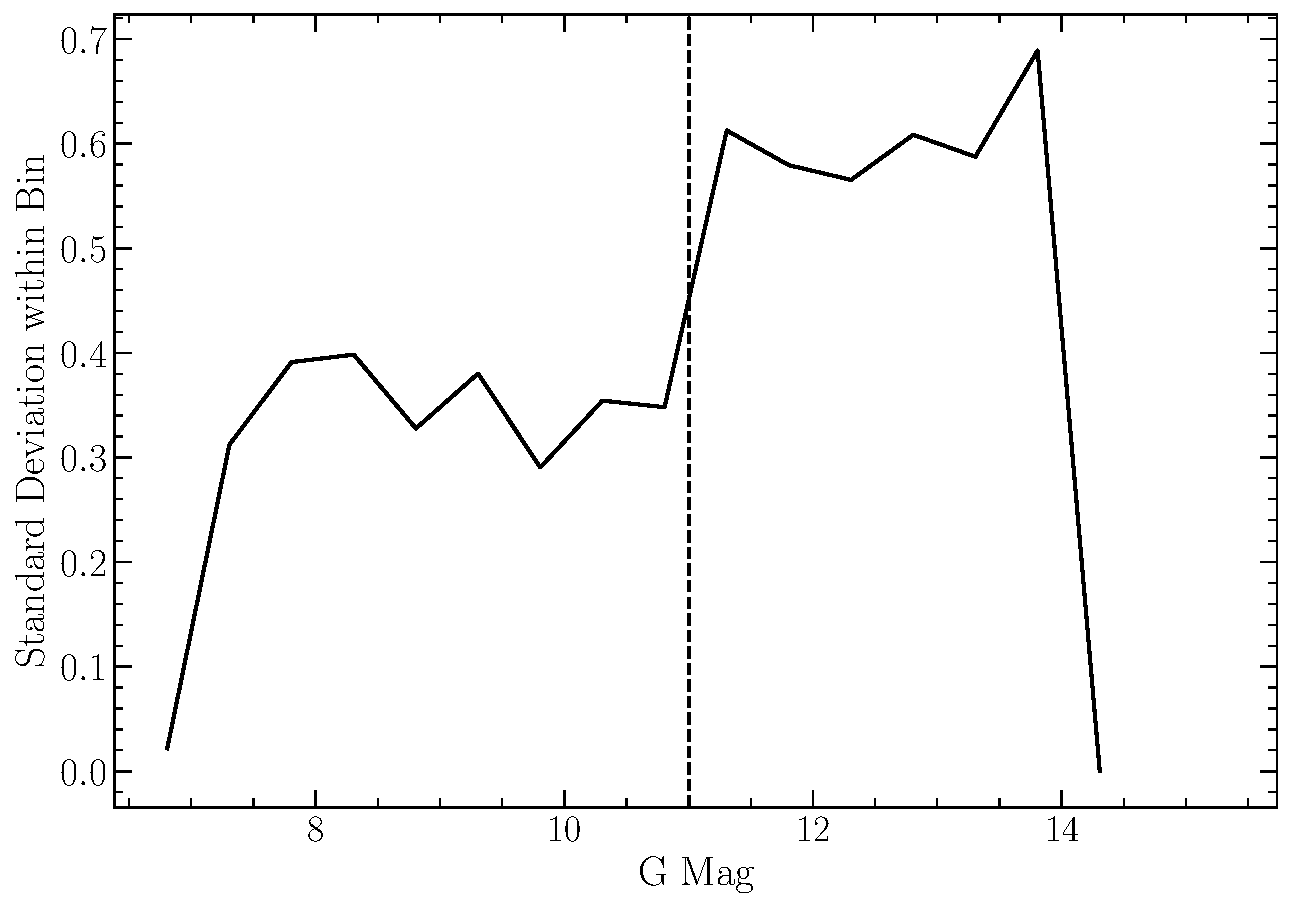
\includegraphics[width=0.45\textwidth]{figures/jaoMagActivity/Deviation.pdf}
  \caption{Standard deviation of Calcium emission data within each bin. Note
  the discontinuity near the Jao Gap Magnitude.}
  \label{fig:deviation}
\end{figure}

\begin{figure}
  \centering
  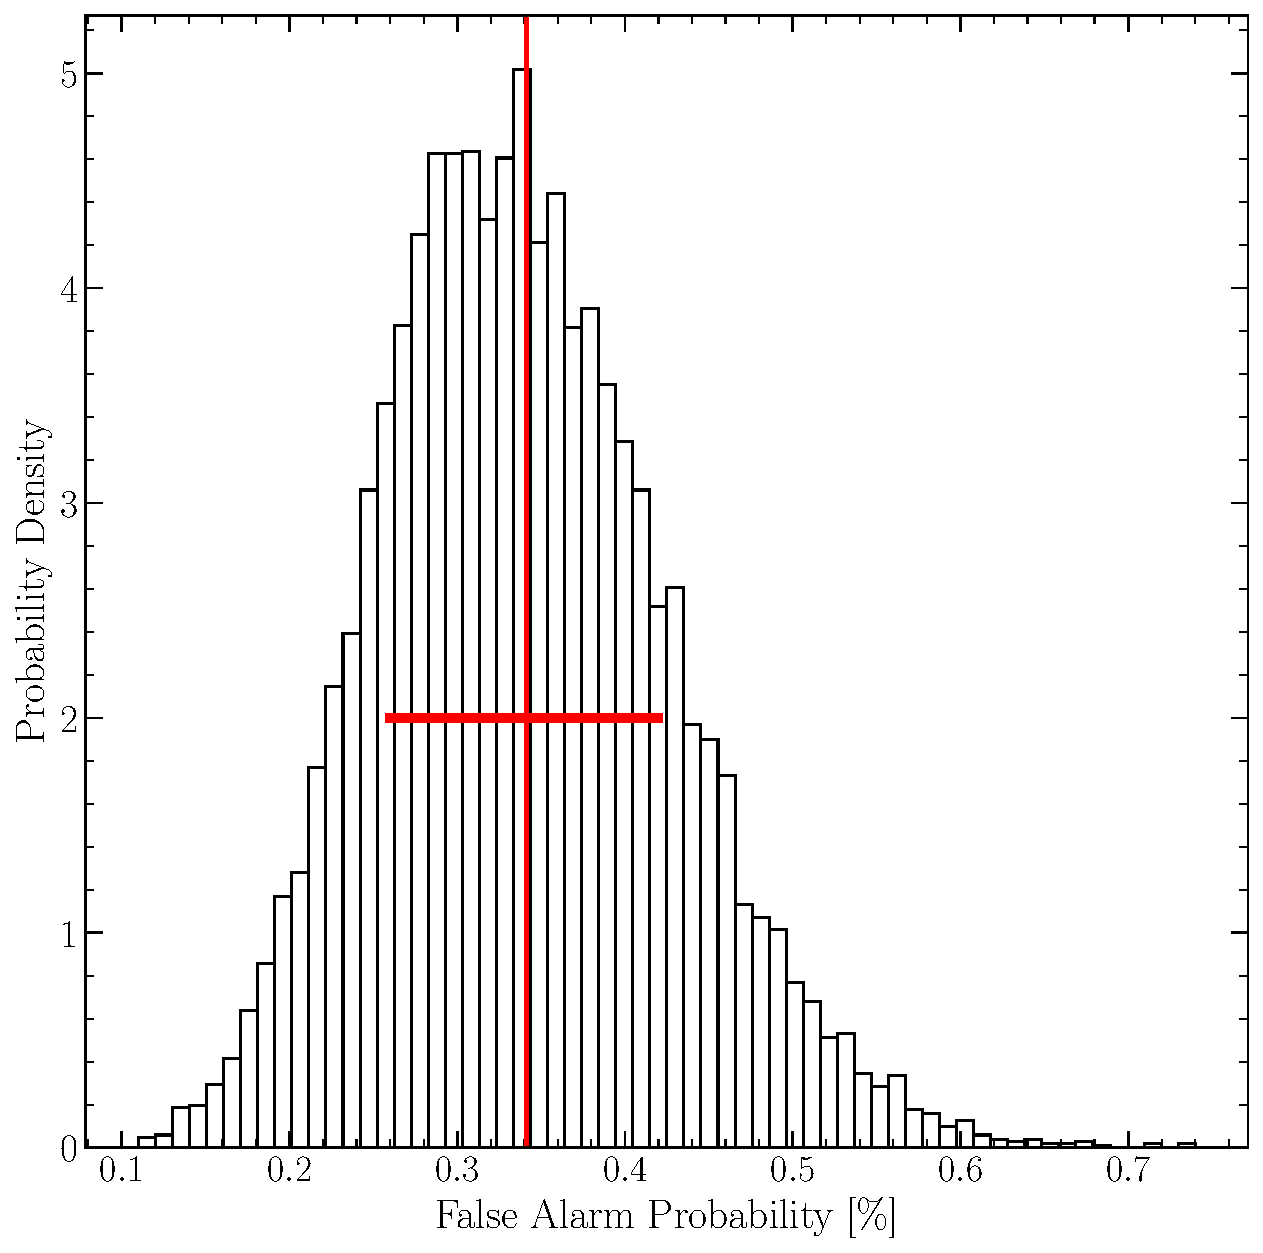
\includegraphics[width=0.45\textwidth]{figures/jaoMagActivity/fpDist.pdf}
  \caption{Probability distribution of the false alarm probability for the
  discontinuity seen in Figure \ref{fig:deviation}. The mean of this
  distribution is $0.341\%\pm^{0.08}_{0.08}$.}
  \label{fig:dist}
\end{figure}

This rapid increase star-to-star variability would only arise due purely to
noise $0.3\pm0.08$ percent of the time and is therefore likely either a true
effect or an alias of some sample bias. {\color{red} COME BACK TO HERE TO FLUSH
OUT SAMPLE BIAS SECTION.}

If the observed increase in variability is not due to a sample bias and rather
is a physically driven effect then there is an obvious similarity between these
findings and those of \citep{Jao2023}. Specifically we find a increase in
variability just below the magnitude of the gap. Moreover, this variability
increase is primarily driven by an increase in the number of low activity stars
(as opposed to an increase in the number of high activity stars). We can
further investigate the observed change in variability for only low activity
stars by filtering out those stars at or above the saturated threshold for
magnetic activity. \citet{Boudreaux2022} identify $\log(R'_{HK}) = -4.436$ as
the saturation threshold. We adopt this value and filter out all stars where
$\log(R'_{HK}) \geq -4.436$. Applying the same analysis to this reduced dataset
as was done to the full dataset we still find a discontinuity at the same
location (Figure \ref{fig:reduced}). This discontinuity is of a smaller
magnitude and consequently is more likely to be due purely to noise, with a
$7\pm0.2$ percent false alarm probability. This false alarm probability is
however only concerned with the first point after the jump in variability. If
we consider the false alarm probability of the entire high variability region
then the probability that the high variability region is due purely to noise
drops to $1.4\pm0.04$ percent.

\begin{figure}
  \centering
  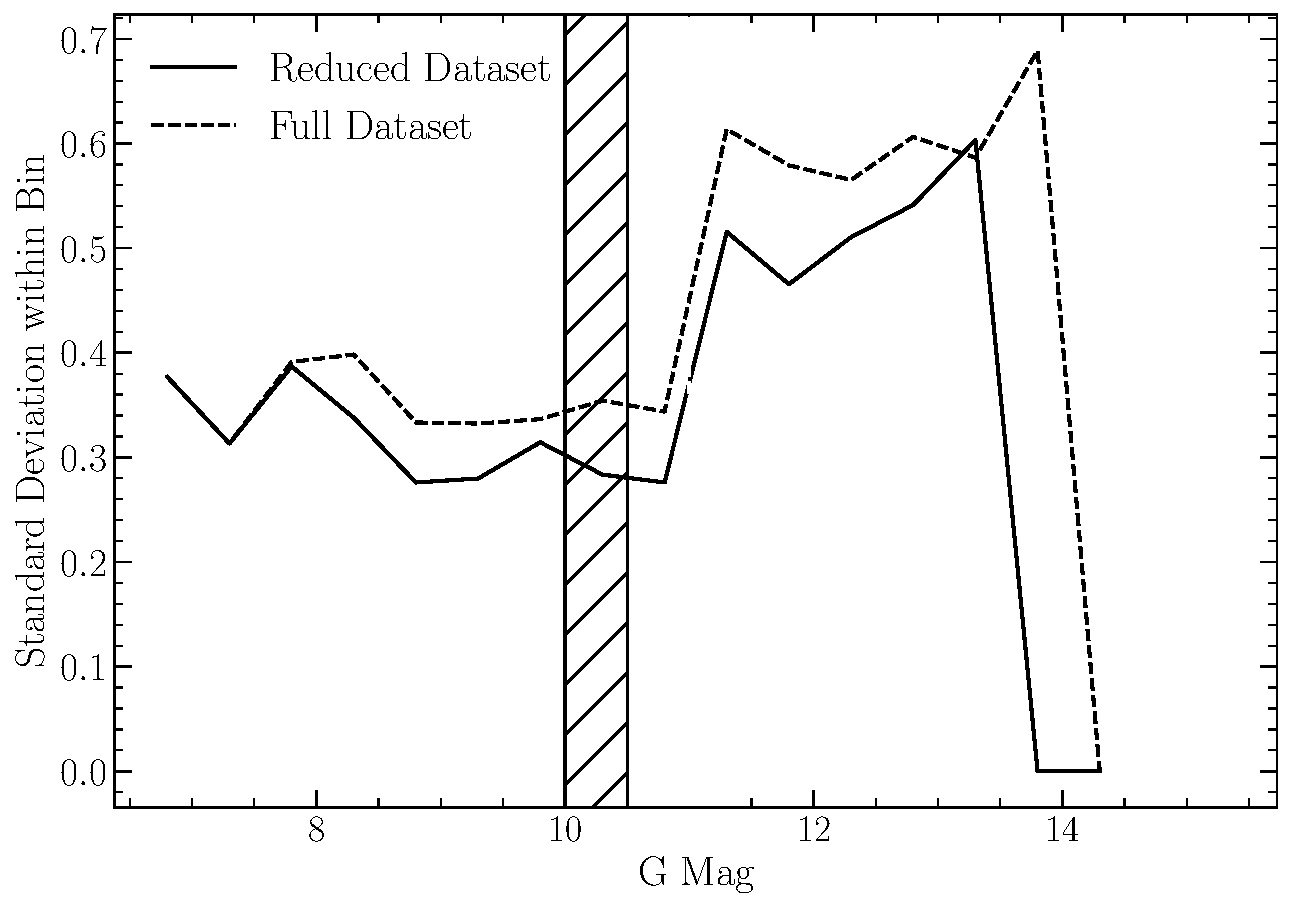
\includegraphics[width=0.45\textwidth]{figures/jaoMagActivity/ReducedDeviation.pdf}
  \caption{Spread in the magnetic activity metric for the merged sample with
  any stars $\log(R'_{HK}) > -4.436$ filtered out.}
  \label{fig:reduced}
\end{figure}

We observe a strong, likely statistically significant, discontinuity in the
star-to-star variability of Ca II K \& K emission just below the magnitude
of the Jao Gap. However, modeling is required to determine if this discontinuity
may be due to the same underlying physics.

While the observed increase in variability seen here does not seem to be
coincident with the Jao Gap --- instead appearing to be approximately 0.5 mag
fainter, in agreement with what is observed in \citet{Jao2023} --- a number of
complicating factors prevent us from falsifying that the these two features are
not coincident. \citeauthor{Jao2023} find, similar to the results presented
here, that the paucity of $H\alpha$ emission originates just below the gap.
Moreover, we use a 0.5 magnitude bin size when measuring the star-to-star
variability which injects error into the positioning of any feature in
magnitude space. We can quantify the degree of uncertainty the magnitude bin
choice injects by conducting Monte Carlo trials where bins are randomly shifted
redder or bluer. We conduct 10,000 trials where each trial involves sampling a
random shift to the bin start location from a normal distribution with a
standard deviation of 1 magnitude. For each trial we identify the discontinuity
location as the maximum value of the gradient of the standard deviation
(effectively this is just the derivative of \ref{fig:reduced}). Some trials
result in the maximal value lying at the 0th index of the magnitude array due
to edge effects, these trials are rejected (and account for 11\% of the
trials). The uncertainty in the identified magnitude of the discontinuity due
to the selected start point of the magnitude bins reveals a $1\sigma = \pm$0.32
magnitude uncertainty in the location of the discontinuity (Figure
\ref{fig:GapLocationMC}). Finally, all previous studies of the M dwarf gap
\citep{Jao2018, Feiden2022, Mansfield2021, Boudreaux2022, Jao2023} demonstrate
that the gap has a color dependency, shifting to fainter magnitudes as the
population reddens and consequently an exact magnitude range is ill-defined.
Therefore we cannot falsify the model that the discontinuity in star-to-star activity
variability is coincident with the Jao Gap magnitude.

\begin{figure}
  \centering
  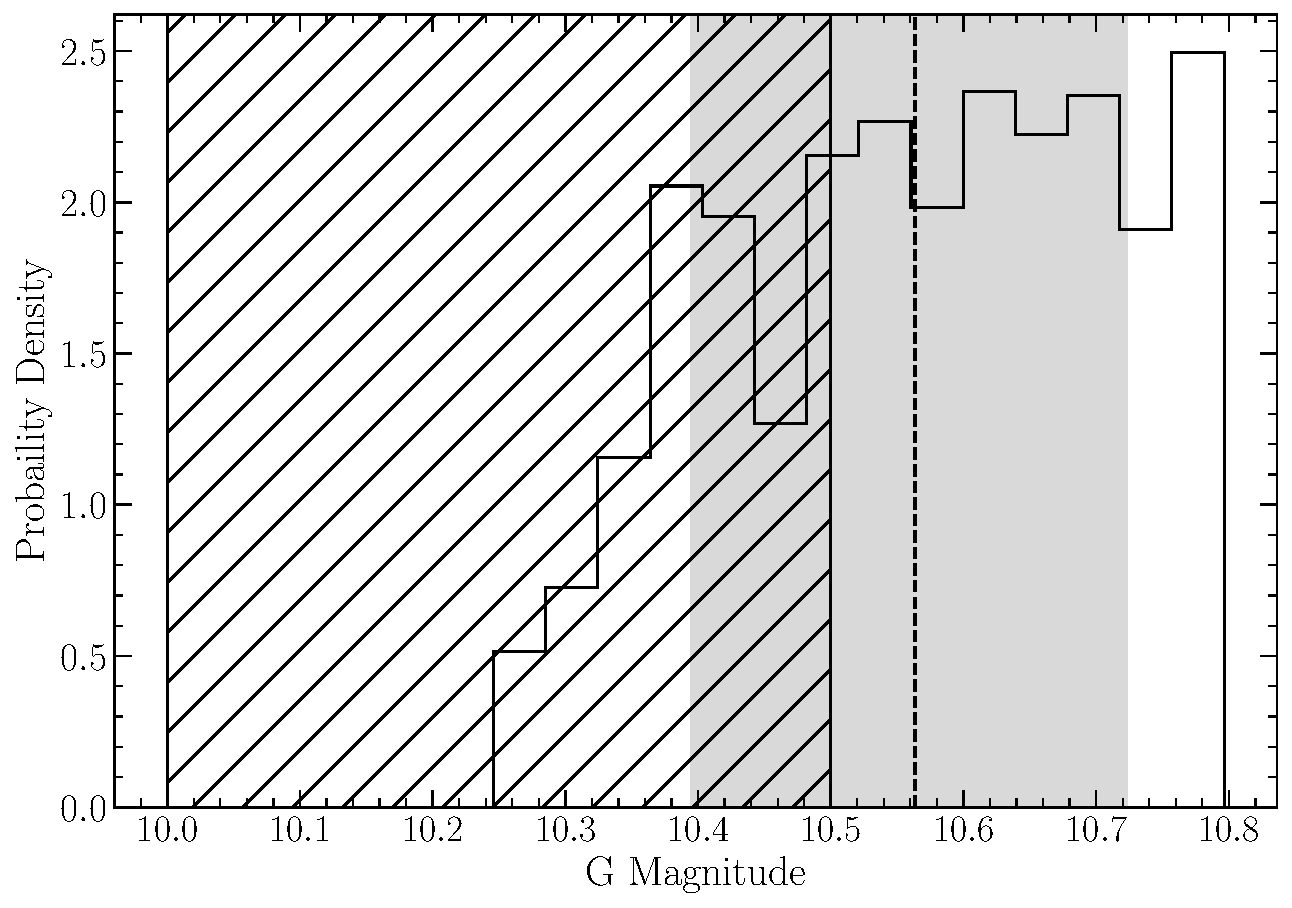
\includegraphics[width=0.45\textwidth]{figures/jaoMagActivity/GapLocationMC.pdf}
  \caption{Probability density distribution of discontinuity location as
  identified in the merged dataset. The dashed line represents the mean of the
  distribution while the shaded region runs from the 16th percentile to the
  84th percentile of the distribution. This distribution was built from 10,000
  independent samples where the discontinuity was identified as the highest
  value in the gradient of the standard deviation.}
  \label{fig:GapLocationMC}
\end{figure}

\subsection{Rotation}
Following the process described in \citet{023AJ....165..192G}, we first put the
dataset through \texttt{stella} \citep{FeinsteinFlare2020,FeinsteinStella2020},
a convolutional neural network that trains a multitude of models, given a
different initial seed, on TESS 2-min cadence. In this case, we also used an
ensemble of 100 models to optimize the gains. \texttt{stella} identifies flares
given a score of 0 to 1, here we use a score of 0.5 and above as flare
identification. Furthermore, we also bin the data from a 2-min to 10-min
cadence using \texttt{lightkurve}'s binning function
\citep{LightkurveCollaborationLightkurve2018,GeertBarentsenKeplerGO2020}. Not
only does this help further reduce any flaring-contribution that might have
been missed by \texttt{stella}\footnote{This is relevant for flares that are
misshapen at the start or break in the dataset due to missing either the
ingress or egress.}, but it also optimizes computational efficiency.
Subsequently, we calculate residuals by subtracting the model from the data,
retaining data with residuals smaller than 4 times the root-mean-square.

As M dwarfs often exhibit non-sinusoidal and quasi-periodic rotational
variability, we employ Gaussian processes for modeling based on
\citet{AngusInferring2018} for the subset of M Dwarfs with no fiducial periods.
The \texttt{starspot} \ package is adapted for light curve analysis
\citep{AngusRuthAngus2021,https://doi.org/10.5281/zenodo.7697238} and
accessible at (HAVEN'T DONE IT YET-AYLIN). Our Gaussian process kernel function
incorporates two stochastically-driven simple harmonic oscillators,
representing primary ($P_\textrm{rot}$) and secondary ($P_\textrm{rot}/2$)
rotation modes. First, we implement the Lomb-Scargle periodogram within
\texttt{starpot} to initially estimate the period. After which, we create a
maximum a posteriori (MAP) fit using \texttt{starspot} to generate a model for
stellar rotation. To obtain the posterior of the stellar rotation model, we use
Markov Chain Monte Carlo (MCMC) sampling using the \texttt{pymc3} package
\citep{SalvatierProbabilistic2016} within our adapted \texttt{starspot}
version. 

ANALYSIS PART YET TO BE DETERMINED.

\subsection{Limitations}
There are two primary limitation of our dataset. First, we only have
{\color{red}232 stars} in our dataset limiting the statistical power of our
analysis. This is primarily due to the relative difficulty of obtaining Ca II
H\&K measurements compared to obtaining $H\alpha$ measurements. Reliable
measurements require both high spectral resolutions ({\color{red} R $\sim$
XXXXXX}) and a comparatively blue wavelength range \footnote{wrt. too what many
spectrographs cover. There is no unified resource listing currently
commissioned spectrographs; however, it is somewhat hard to source glass which
transmits well at H\&K wavelengths limiting the lower wavelength of most
spectrographs.}.

Additionally, the sample we do have does not extend to as low mass as would be
ideal. This presents a degeneracy between two potential causes for the observed
increased star-to-star variability. One option, as presented above and
elaborated on in the following section, is that this is due to kissing
instabilities. However, another possibility is that this increased variability
is intrinsic to the magnetic fields of fully convective stars. There is limited
discussion in the literature of the latter effect; however, \citet{Shulyak2019}
present estimated magnetic field strengths for 47 M dwarfs, spanning a larger
area around the convective transition region and their dataset does not
indicate a inherently increased variability for fully convective stars
({\color{red} fully confirm this, not just visually}).

\section{Conclusion}\label{sec:conclusion}
It is, at this point, well established that the Jao Gap may provide a unique view of the interiors of stars for which other probes, such as seismology, fail. However, it has only recently become clear that the Gap may lend insight into not just structural changes within a star but also into the magnetic environment of the star.
\citet{Jao2023} presented evidence that the physics driving the Gap might additionally result in a paucity of H$\alpha$ emission. These authors propose potential physical mechanisms which could explain this paucity, including the core of the star acting as an angular momentum sink during mixing events.

Here we have expanded upon this work by probing the degree and variability of
Calcium II H\&K emission around the Jao Gap. We lack the same statistical
power of \citeauthor{Jao2023}'s sample; however, by focusing on the
star-to-star variability within magnitude bins we are able to retain
statistical power. We find that there is an anomalous increase in variability
at a G magnitude of $\sim 11$. This is only slightly below the observed mean gap magnitude.

Additionally, we propose a simple model to explain this variability. Making the
assumption that the periodic convective mixing events will have some small but
random effect on the overall magnetic field strength we are able to
qualitatively reproduce the increase activity spread in a synthetic population
of stars. 


